\documentclass[12pt]{report}

% ==== Essential Packages ====
\usepackage{fontspec}
\usepackage{graphicx}
\usepackage{geometry}
\usepackage{float}
\usepackage{caption} 
\usepackage{array}
\usepackage{tabularx} 
\usepackage{fancyhdr}
\usepackage{changepage}
\usepackage[round]{natbib}
\usepackage{enumitem}
\usepackage[colorlinks=true, linkcolor=blue, urlcolor=blue, citecolor=blue]{hyperref}

% ==== Page Layout ====
\geometry{
  a4paper,
  top=1.5cm,
  bottom=2.0cm,
  left=2.0cm,
  right=2.0cm
}

% ==== Font Setup ====

% Khmer fonts
\newfontfamily\khmerfont{Khmer OS Muol Light}       % for headings
\newfontfamily\khmernormal{Khmer OS Content}        % for body text


% English font
\newfontfamily\englishfont{Times New Roman}

% Enable proper line breaking for Khmer
\XeTeXlinebreaklocale "khmer"
\XeTeXlinebreakskip = 0pt plus 1pt

% Center chapter titles
\usepackage{titlesec}
\titleformat{\chapter}[display]
  {\normalfont\huge\bfseries\centering}
  {\chaptertitlename\ \thechapter}{5pt}{\Huge}

\title{}
\author{}
\date{}

\begin{document}

% === Title Pages ===
\begin{titlepage}
    \centering
    \vspace*{1cm}

    \begin{minipage}{0.25\textwidth}
        
\includegraphics[width=3.5cm]{figures/RUPP.jpg}
    \end{minipage}
    \hfill
    \begin{minipage}{0.65\textwidth}
        \raggedright
        {\khmerfont\fontsize{16pt}{20pt}\selectfont សាកលវិទ្យាល័យភូមិន្ទភ្នំពេញ\\[0.6em]}
        {\large\bfseries ROYAL UNIVERSITY OF PHNOM PENH}
    \end{minipage}

    \vspace{2cm}

    \begin{minipage}{0.9\textwidth}
        \centering
        {\khmerfont\fontsize{12pt}{20pt}\selectfont ការស្រាវជ្រាវវិធីសាស្ដ្រថ្មី  សម្រាប់កំណត់សម្គាល់អត្ថបទអក្សរខ្មែរទូទៅ នឹងបានប្រើប្រាស់ស្ថាបត្យកម្ម {\englishfont\textbf{Craft}} ជាមួយនឹង {\englishfont\textbf{TrOCR}}\\[0.4em]}
        {\englishfont\fontsize{15pt}{20pt}\selectfont\bfseries A novel End-to-End approach for General Khmer Text \par}
        {\englishfont\fontsize{15pt}{20pt}\selectfont\bfseries Recognition using Craft with TrOCR Architecture \par}
    \end{minipage}

    \vspace{3.0cm}

    {\englishfont\fontsize{16pt}{20pt}\selectfont Mr. Vitou Soy\par}

    \vspace{3.0cm}

    {\englishfont\fontsize{16pt}{20pt}\selectfont A Thesis\par}
    \vspace{0.5cm}
    {\large In Partial Fulfilment of the Requirement for the Degree of\par}
    {\large Bachelor of Engineering in Information-Technology-Engineering\par}
    

    \vspace{2.5cm}

    {\englishfont
    \begin{center}
        \begin{tabular}{ll}
            {Examination committee:} & Mr. Sokchea Kor (Advisor) \\
                                    & Mr. Chanpiseth Chap (committee) \\
                                    & Mrs. Daly Chea (committee)\\
                                    & Dr. \dotfill
        \end{tabular}
    \end{center}
    }

    \vfill
    {\Large\bfseries June 2025\par}
\end{titlepage}

\thispagestyle{empty}

\begin{titlepage}
    \centering
    \vspace*{1cm}

    \centering
    \begin{minipage}{0.9\textwidth}
        \centering
        {\khmerfont\fontsize{16pt}{20pt}\selectfont សាកលវិទ្យាល័យភូមិន្ទភ្នំពេញ\\[0.6em] \par}
        {\englishfont\fontsize{12.5pt}{20pt}\selectfont\bfseries\textbf{ROYAL UNIVERSITY OF PHNOM PENH}}
    \end{minipage}
    

    \vspace{2cm}

    \begin{minipage}{0.9\textwidth}
        \centering
        {\khmerfont\fontsize{14pt}{20pt}\selectfont ការបំប្លែងរូបភាពឯកសារទៅជាអក្សរកែប្រែបានទៅលើភាសាខ្មែរនិង អង់គ្លេស ដោយប្រើប្រាស់ ម៉ូដែល {\englishfont\textbf{Craft}} ជាមួយនឹង {\englishfont\textbf{TrOCR}}\\[0.4em]}
        {\englishfont\fontsize{14pt}{20pt}\selectfont\bfseries An End-to-End approach for Khmer \& English Text \par}
        {\englishfont\fontsize{14pt}{20pt}\selectfont\bfseries Recognition using Craft with TrOCR Architecture \par}
    \end{minipage}

    \vspace{3.0cm}

    {\englishfont\fontsize{14pt}{20pt}\selectfont A Thesis\par}
    \vspace{0.5cm}
    {\englishfont\fontsize{13pt}{20pt}\selectfont\large In Partial Fulfilment of the Requirement for the Degree of\par}
    {\englishfont\fontsize{13pt}{20pt}\selectfont\large Bachelor of Engineering in Information Technology Engineering\par}
    

    \vspace{3.0cm}

    {\englishfont\fontsize{14pt}{20pt}\bfseries\textbf\selectfont Vitou Soy\par}

    

    

    \vspace{2.5cm}

    {\englishfont
    \begin{center}
        \begin{tabular}{ll}
            {Examination committee:} & Mr. Sokchea Kor \\
                                    & Mr. Chanpiseth Chap\\
                                    & Mrs. Daly Chea\\
                                    & Dr. \dotfill
        \end{tabular}
    \end{center}
    }

    \vfill
    {\englishfont\fontsize{20pt}{20pt}\Large\bfseries June 2025\par}
\end{titlepage}

\thispagestyle{empty}

% === Preliminary Pages ===
\thispagestyle{plain}
\begin{adjustwidth}{0.2cm}{0.2cm}


    % supervisor statement
    \begin{center}
        {\englishfont\fontsize{14pt}{21pt}\selectfont \textbf{SUPERVISOR's RESEARCH SUPERVISION STATEMENT} \par}
    \end{center}
    \phantomsection
    \label{supervisor-statement}

    \vspace{1cm}
    
    \englishfont\large
    \begin{flushleft}
    Name of program: Khmer Studies\par
    Name of candidate: Vitou Soy\par
    \end{flushleft}

    \vspace{1cm}
    
    \englishfont\large
    \begin{flushleft}
    Title of research report: A novel End-to-End approach for General Khmer Text
    Recognition using Craft with TrOCR Architecture\par
    \end{flushleft}

    \vspace{1cm}
    \setlength{\parindent}{0pt}
    This is to certify that the research carried out for the above titled master's
    research report was completed by the above named candidate under my direct
    supervision. This thesis material has not been used for any other degree. The
    candidate has demonstrated strong research capabilities and independence in
    developing novel approaches for Khmer text recognition. The research
    methodology, implementation, and results are original contributions to the field
    of Khmer OCR technology. I have provided guidance and oversight throughout
    the research process while allowing the candidate to explore innovative
    solutions.\par

    \vspace{1cm}
    \begin{flushleft}
    Supervisor's name: Sokchea Kor\par
    \vspace{0.1cm}
    Supervisor's signature:……………………\par
    \vspace{0.1cm}
    Date……………………………………………\par
    \end{flushleft}

\end{adjustwidth}
\newpage

\thispagestyle{plain}
\begin{adjustwidth}{0.2cm}{0.2cm}

    % Khmer Abstract
    \begin{center}
        {\khmerfont\fontsize{15pt}{25pt}\selectfont សង្ខេបសេចក្ដី \par}
    \end{center}
    \phantomsection
    \label{khmer-abstract}
    \vspace{0.5cm}
    \khmernormal
    \small
    ក្នុងសហគមន៍បច្ចេកវិទ្យាព័ត៌មានសម័យថ្មី ការចាប់យកអត្ថបទចេញពីរូបភាព  – [ OCR ]
    (Optical Character Recognition) ក្លាយជាបច្ចេកវិទ្យាសំខាន់មួយដែលត្រូវបានប្រើប្រាស់
    យ៉ាងទូលំទូលាយ សម្រាប់បំលែងឯកសារសរសេរ ឬរូបភាពអក្សរឱ្យទៅជាអត្ថបទ អេឡិចត្រូនិច (digital text)។ 
    ការអភិវឌ្ឍ OCR សម្រាប់ភាសាខ្មែរ តែងតែប្រឈមនឹងបញ្ហាជាច្រើន ដោយសារកង្វះនៃប្រភពទិន្នន័យ 
    និងឯកសារសម្រាប់ train AI model។ ដើម្បីដោះស្រាយបញ្ហានេះ យើងបានបង្កើតទិន្នន័យសិប្បនិម្មិត 
    (Synthetic Dataset) ដោយប្រើវិធីសាស្ត្របច្ចេកទេសកម្រិតខ្ពស់។\par
    
    ក្នុងដំណើរការបង្កើតទិន្នន័យសិប្បនិម្មិត (Synthetic Dataset) រួមមាន៖
    \begin{itemize}
        \item វិធីសាស្ដ្រក្នុងការប្រមូលអត្ថបទចេញពីអ៊ីនធឺណិត មានដូចខាងក្រោម (Scrape data) ៖
        \begin{itemize}
            \item ដំណាក់កាលទីមួយ៖ យើងបានប្រមូលអត្ថបទចេញពី khsearch.com, Chuon-Nath-Dictionary, Alpha-Word, Google-Word, និងចុងក្រោយគឺ Huggingface.com ។
            \item ដំណាក់កាលទីពីរ៖ យើងបានសម្អាត ទិន្នន័យទាំងអស់នោះ ឆ្លងកាត់ដំណើរការ ដូចជា លុបចោលតួរអក្សរណាដែលមិនសូវមាន វត្តមាននៅលើ រូបភាព ញឹកញាប់ និងបានលុបចោល តួរអក្សរណាដែល Fonts renders អត់ចេញ។
            \item ដំណាក់កាលទីបី៖ ដំណាក់កាលមួយនេះ យើងបានធ្វើការ កាត់ប្រយោគទាំងអស់នោះ ជាពាក្យៗ ដោយប្រើប្រាស់ library ឈ្មោះ khmer-nltk
            \item ដំណាក់កាលទីបួន៖ ចុងក្រោយ ក៏បានរៀបចំជា ប្រយោគដែល មានប្រវែង Random ពី ១ អក្សរ រហូតដល់ ១១០ អក្សរ ។
        \end{itemize}
        \item បង្កើតរូបភាពដោយអនុវត្តតាមលក្ខខណ្ឌខាងក្រោម ៖ 
        \begin{itemize}
            \item ផ្ទៃខាងក្រោយចៃដន្យ (Apply Different backgrounds)
            \item បំពាក់ពុម្ពអក្សរផ្សេងៗគ្នា (Apply Different fonts)
            \item Noise: \texttt{gaussian\_noise}, \texttt{salt\_pepper\_noise}, \texttt{speckle\_noise}, \texttt{blur}
            \item បង្វិលអក្សរបន្តិច (random rotation text)
            \item បញ្ចូល Margin Randomly (1, 5) pixels
        \end{itemize}
        \item សរុបមកយើងបានបង្កើត Data ជាង ៤ លាន records សម្រាប់ train OCR model
    \end{itemize}
    \par
    
    Architecture OCR ត្រូវបានបែងចែកជា ២ ផ្នែក៖ \textbf{Text Detection} និង \textbf{Text Recognition}:\par
    
    \textbf{Text Detection}: យើងប្រើម៉ូដែល \textbf{CRAFT} ដោយបានធ្វើការ Train ឡើងវិញដោយ បាន annotation ទៅលើ 
    លើរូបភាពប្រហែល ៥០០ images និងសរុបចំនួន bounding box ជាង ១០,០០០ boxes។\par
    
    \textbf{Text Recognition}: យើងប្រើ \textbf{TrOCR base model} ចេញពី Microsoft (មាននៅក្នុង Hugging Face) ហើយបាន
    fine-tune ទៅលើ dataset ខ្មែរសិប្បនិម្មិត (Synthetic Dataset) ដើម្បីបង្កើនសមត្ថភាពក្នុងការសម្គាល់អក្សរខ្មែរ។\par
    
    លទ្ធផលសិក្សាបានបង្ហាញថា OCR របស់ពួកយើងអាចសម្គាល់អត្ថបទចេញពីរូបភាព បានដោយភាពត្រឹមត្រូវលើសពី ៩០\%។ 
    ដូច្នេះ ការសិក្សានេះបង្ហាញអំពីសក្តានុពលនៃការបង្កើត dataset និងការប្រើម៉ូដែលជំនាន់ថ្មី ដើម្បីអភិវឌ្ឍន៍ OCR ភាសាខ្មែរឱ្យមានប្រសិទ្ធភាពកាន់តែខ្ពស់។
    វាមានសមត្ថភាព អាចចាប់យកអត្ថបទមិនត្រឹមតែពាក្យខ្លីៗ ប៉ុណ្ណោះទេ តែវាក៏អាចធ្វើការចាប់យក ដូចជា មួយតួអក្សរដោយមួយតួអក្សរ, ពាក្យដោយពាក្យ, ប្រយោគដោយប្រយោគ រហូតដល់ មួយប្រយោគវែង ១១០ តួអក្សរថែមទៀតផង ។ ហើយលើសពីនោះទៀត វាក៏អាចធ្វើការ កំណត់សម្គាល់ទៅលើ ពីរ ភាសាចម្បង ទាំងភាសាខ្មែរ និងភាសាអង់គ្លេស ។    
    \vspace{2cm}
    
    % English Abstract
    \begin{center}
        {\bfseries\LARGE Abstract \par}
    \end{center}
    \phantomsection
    \label{abstract}
    \vspace{0.5cm}
    \englishfont
    \large
    
    OCR technology continues to evolve rapidly, but Khmer text 
    recognition still presents challenges—mainly because of the 
    limited availability of high-quality training data. In this work, 
    we introduce an end-to-end OCR approach for both Khmer and English text, 
    tailored to work well even under low-resource conditions. Our pipeline combines 
    reliable text detection and advanced recognition techniques, designed to reflect real-world multilingual usage in Cambodia.

    We began by manually collecting a dataset of 1,000 real-world images, 
    carefully annotating 13,200 text-line bounding boxes in both Khmer and English. 
    This gave us a strong foundation to train our text detection model using CRAFT, 
    which excels at detecting irregular text regions. Training on our custom-annotated 
    data, the CRAFT model achieved strong performance, with 90\% recall, 89\% precision, 
    and an F1-score of 86.8\%. These results show that with focused annotation efforts, 
    high-quality detection is achievable even without large public datasets.
    
    To further improve the system’s performance and handle a wider variety of input, 
    we generated a synthetic training dataset using a text-to-image method. We 
    collected a large corpus of Khmer and English sentences from the web and used 
    this to create thousands of synthetic images simulating different fonts, layouts, 
    and noise patterns. This synthetic data expanded the diversity of our training 
    set and allowed the model to better generalize to unseen real-world samples.
    
    For the recognition stage, we used TrOCR—a transformer-based architecture built 
    for OCR tasks. However, the original TrOCR processor was not designed to support 
    Khmer text and could not correctly interpret the language. To address this, 
    we customized the processor so that it could properly tokenize and decode Khmer 
    characters. This modification was essential to ensure that the model could 
    understand and accurately transcribe Khmer script.
    
    After training on both real and synthetic data, our TrOCR-based recognition model 
    showed strong results on real-world test images: a character error rate (CER) 
    of 0.02 overall, with 0.04 for Khmer, 0.01 for English, and 0.06 for lines 
    containing both languages.
    
    One of the key motivations behind this work is the increasing use of English 
    in Cambodia. While Khmer remains the national language, English is now widely 
    used as a second language and often appears alongside Khmer in signs, documents, 
    and digital platforms. By building a system that supports both languages, 
    we aim to match the multilingual nature of everyday text in Cambodia.
    
    Finally, unlike most academic research that never reaches real-world usage, 
    we’ve made our OCR system publicly accessible through a production-ready API. 
    This allows others to test and integrate the model into their own applications, 
    bridging the gap between research and practical deployment. According to recent 
    studies, nearly 80\% of research models never get deployed or made accessible—our 
    goal was to break that trend. By turning our model into a usable, open API, 
    we ensure that the results of this work are not only measurable in papers 
    but also usable by the community.


    
    \end{adjustwidth}
\newpage

\thispagestyle{plain}
\begin{adjustwidth}{0.2cm}{0.2cm}

% supervisor statement
\begin{center}
    {\englishfont\fontsize{14pt}{21pt}\selectfont \textbf{CANDIDATE'S STATEMENT} \par}
\end{center}
\label{candidate-statement}

\vspace{1cm}
{\englishfont\fontsize{12pt}{18pt}\selectfont \setlength{\parindent}{0pt} TO WHOM IT MAY CONCERN \par}

\vspace{0.5cm}
    \setlength{\parindent}{0pt}
    {\large This is to certify that the dissertation that I, Vitou Soy, hereby present, entitled "Advancing
    Khmer Optical Character Recognition: A Synthetic Data-Driven Approach," for the degree
    of Bachelor of Engineering in Information Technology at the Royal University of Phnom Penh, is
    entirely my own work. Furthermore, it has not been used to fulfill the requirements of any
    other qualification, in the whole or in part, at this or any other University or equivalent
    institution. The research methodology, implementation, and findings represent original con-
    tributions to the field of Khmer OCR technology, particularly in developing novel approaches
    for synthetic data generation and transformer-based text recognition. Through this work, I
    have demonstrated strong research capabilities and independence in addressing the critical
    challenges of Khmer text digitization and recognition.\par}

    \vspace{0.5cm}
    \setlength{\parindent}{0pt}
    {\large No reference to, or quotation from, this document may be made without the written
    approval of the author.\par}
    \vspace{1cm}
    \setlength{\parindent}{0pt}
    {\large Name of Candidate: Vitou Soy\par}
    
    \vspace{0.5cm}
    \setlength{\parindent}{0pt}
    {\large Signed by the candidate: \hspace{1cm}\raisebox{-1ex}{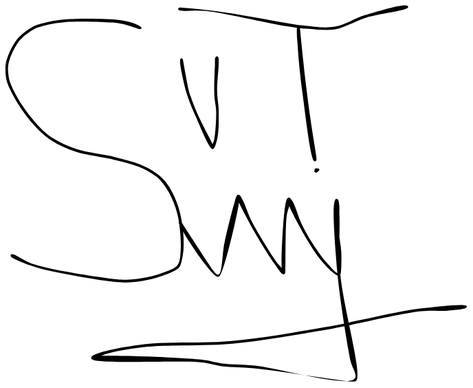
\includegraphics[width=1cm]{figures/sign_cadidate.png}}\hspace{\fill}\par}
    
    \vspace{0.5cm}
    \setlength{\parindent}{0pt}
    {\large Date: \dotfill\par}

    \vspace{1cm}
    \setlength{\parindent}{0pt}
    {\large Name of Supervisor: Mr. Sokchea Kor\par}
    
    \vspace{0.5cm}
    \setlength{\parindent}{0pt}
    {\large Countersigned by the Supervisor: \dotfill\par}
    
    \vspace{0.5cm}
    \setlength{\parindent}{0pt}
    {\large Date: \dotfill\par}

    
\end{adjustwidth}
\newpage

\thispagestyle{plain}
\begin{adjustwidth}{0.2cm}{0.2cm}

    % Acknowledgments
    \begin{center}
        {\englishfont\fontsize{14pt}{21pt}\selectfont \textbf{ACKNOWLEDGMENTS} \par}
    \end{center}
    \phantomsection
    \label{acknowledgements}

    \vspace{1cm}
    \setlength{\parindent}{2em}
    {\large I would like to begin by expressing my sincere gratitude for the opportunity to pursue this research. I am deeply thankful to the Royal University of Phnom Penh for offering such a well-structured academic program within the Faculty of Engineering, which has provided a strong foundation for this success. The comprehensive curriculum, practical exposure, and academic environment have been instrumental in shaping my journey.

    \vspace{0.5cm}
    I am especially grateful to all the faculty members for their dedicated teaching and continuous support throughout my studies. Their commitment to student learning has inspired and guided me significantly. I would also like to thank my classmates for their collaboration, encouragement, and the shared experiences that made this journey memorable.

    \vspace{0.5cm}
    My deepest appreciation goes to my supervisor, Mr. Kor Sokchea, whose expertise, mentorship, and unwavering support have been vital to the completion of this work. He has been not only an exceptional lecturer and supervisor but also a strong supporter at every stage. This research would not have been possible without his guidance.

    \vspace{0.5cm}
    Finally, I want to express my heartfelt thanks to my family for their financial support, constant encouragement, and unconditional love. Their sacrifices and belief in me have been the driving force behind my achievements. I am especially grateful to my sister, who has always believed in me and supported every decision I made—thank you for always standing by my side.

    \par}

\end{adjustwidth}

\newpage

\thispagestyle{plain}
\begin{adjustwidth}{0.2cm}{0.2cm}

    \begin{center}
        {\englishfont\fontsize{14pt}{21pt}\selectfont \textbf{TABLE OF CONTENTS} \par}
    \end{center}
    \phantomsection
    \label{toc}

    \vspace{1cm}

    \setlength{\parindent}{0pt}
    {\large \textbf{Preliminary Pages}\par}
    \vspace{0.3cm}
    {\khmernormal\fontsize{11pt}{16pt}\selectfont មូលន័យសង្ខេប\dotfill\hyperref[khmer-abstract]{{\pageref{khmer-abstract}}}\hspace{0.1cm}\par}
    {\large Abstract\dotfill\hyperref[abstract]{{\pageref{abstract}}}\hspace{0.1cm}\par}
    {\large Supervisor's Research Supervision Statement\dotfill\hyperref[supervisor-statement]{{\pageref{supervisor-statement}}}\hspace{0.1cm}\par}
    {\large Candidate's Statement\dotfill\hyperref[candidate-statement]{{\pageref{candidate-statement}}}\hspace{0.1cm}\par}
    {\large Acknowledgements\dotfill\hyperref[acknowledgements]{{\pageref{acknowledgements}}}\hspace{0.1cm}\par}
    {\large Table of Contents\dotfill\hyperref[toc]{{\pageref{toc}}}\hspace{0.1cm}\par}
    {\large List of Tables\dotfill\hyperref[lot]{{\pageref{lot}}}\hspace{0.1cm}\par}
    {\large List of Figures\dotfill\hyperref[lof]{{\pageref{lof}}}\hspace{0.1cm}\par}
    {\large List of Abbreviations\dotfill\hyperref[loa]{{\pageref{loa}}}\hspace{0.1cm}\par}

    \vspace{0.5cm}
    {\large \textbf{Chapter 1: Introduction}\dotfill\pageref{ch:intro}\par}
    {\large 1.1 Background to the Study\dotfill\pageref{sec:background}\par}
    {\large 1.2 Problem Statement\dotfill\pageref{sec:problem}\par}
    {\large 1.3 Aim and Objectives of the Study\dotfill\pageref{sec:objectives}\par}
    {\large 1.4 Research Questions\dotfill\pageref{sec:questions}\par}
    {\large 1.5 Rationale of the Study\dotfill\pageref{sec:rationale}\par}
    {\large 1.6 Limitations and Scope\dotfill\pageref{sec:limitations}\par}
    {\large 1.7 Structure of the Thesis\dotfill\pageref{sec:structure}\par}

    \vspace{0.5cm}
    {\large \textbf{Chapter 2: Literature Review}\dotfill\pageref{ch:literature}\par}
    {\large 2.1 Overview\dotfill\pageref{sec:ocr-overview}\par}
    {\large 2.2 Definition of Optical Character Recognition (OCR)\dotfill\pageref{sec:ocr-definition}\par}

    \vspace{0.5cm}
    {\large \textbf{Chapter 3: Dataset Construction}\dotfill\pageref{ch:dataset}\par}
    {\large 3.1 Text Source Collection\dotfill\pageref{sec:text-source}\par}
    {\large \hspace{1cm}3.1.1 Khmer Websites and Dictionaries\dotfill\pageref{subsec:websites}\par}
    {\large \hspace{1cm}3.1.2 Online NLP Resources and Tools\dotfill\pageref{subsec:nlp-tools}\par}
    {\large 3.2 Text Cleaning and Preprocessing\dotfill\pageref{sec:preprocessing}\par}
    {\large \hspace{1cm}3.2.1 Removal of Invalid Characters and Whitespace\dotfill\pageref{subsec:cleaning}\par}
    {\large \hspace{1cm}3.2.2 Unicode Normalization\dotfill\pageref{subsec:unicode}\par}
    {\large 3.3 Sentence Segmentation and Reconstruction\dotfill\pageref{sec:segmentation}\par}
    {\large \hspace{1cm}3.3.1 Tokenization Using khmer-nltk\dotfill\pageref{subsec:tokenization}\par}
    {\large \hspace{1cm}3.3.2 Sentence Length Variation\dotfill\pageref{subsec:length}\par}
    {\large 3.4 Image Generation Pipeline\dotfill\pageref{sec:generation}\par}
    {\large \hspace{1cm}3.4.1 Font and Background Selection\dotfill\pageref{subsec:fonts}\par}
    {\large \hspace{1cm}3.4.2 Noise Injection Techniques\dotfill\pageref{subsec:noise}\par}
    {\large \hspace{1cm}3.4.3 Image Rotation and Margin Augmentation\dotfill\pageref{subsec:augmentation}\par}
    {\large 3.5 Dataset Statistics and Format\dotfill\pageref{sec:statistics}\par}
    {\large 3.6 Comparison with Existing Datasets\dotfill\pageref{sec:comparison}\par}

    \vspace{0.5cm}
    {\large \textbf{Chapter 4: Experiments}\dotfill\pageref{ch:experiments}\par}
    {\large 4.1 Experimental Environment and Tools\dotfill\pageref{sec:environment}\par}
    {\large 4.2 Model Architecture and Configuration\dotfill\pageref{sec:architecture}\par}
    {\large \hspace{1cm}4.2.1 CRAFT for Text Detection\dotfill\pageref{subsec:craft}\par}
    {\large \hspace{1cm}4.2.2 TrOCR for Text Recognition\dotfill\pageref{subsec:trocr}\par}
    {\large 4.3 Training Methodology\dotfill\pageref{sec:training}\par}
    {\large \hspace{1cm}4.3.1 Fine-tuning CRAFT on Annotated Images\dotfill\pageref{subsec:craft-training}\par}
    {\large \hspace{1cm}4.3.2 Fine-tuning TrOCR on Synthetic Dataset\dotfill\pageref{subsec:trocr-training}\par}
    {\large 4.4 Evaluation Metrics\dotfill\pageref{sec:metrics}\par}
    {\large \hspace{1cm}4.4.1 Detection Metrics (Precision, Recall)\dotfill\pageref{subsec:detection-metrics}\par}
    {\large \hspace{1cm}4.4.2 Recognition Metrics (Accuracy, CER, WER)\dotfill\pageref{subsec:recognition-metrics}\par}
    {\large 4.5 Baseline and Benchmark Comparison\dotfill\pageref{sec:benchmark}\par}

    \vspace{0.5cm}
    {\large \textbf{Chapter 5: Results and Analysis}\dotfill\pageref{ch:results}\par}
    {\large 5.1 Text Detection Results\dotfill\pageref{sec:detection-results}\par}
    {\large \hspace{1cm}5.1.1 Quantitative Metrics\dotfill\pageref{subsec:quantitative}\par}
    {\large \hspace{1cm}5.1.2 Qualitative Visual Examples\dotfill\pageref{subsec:qualitative}\par}
    {\large 5.2 Text Recognition Results\dotfill\pageref{sec:recognition-results}\par}
    {\large \hspace{1cm}5.2.1 Accuracy on Character, Word, Sentence Levels\dotfill\pageref{subsec:accuracy}\par}
    {\large \hspace{1cm}5.2.2 Performance Across Sentence Lengths\dotfill\pageref{subsec:performance}\par}
    {\large 5.3 Khmer vs. English Performance\dotfill\pageref{sec:comparison-results}\par}
    {\large 5.4 Error Analysis and Failure Cases\dotfill\pageref{sec:error-analysis}\par}
    {\large 5.5 System Robustness and Generalization\dotfill\pageref{sec:robustness}\par}

    \vspace{0.5cm}
    {\large \textbf{Chapter 6: Discussion}\dotfill\pageref{ch:discussion}\par}
    {\large 6.1 Effectiveness of Synthetic Data\dotfill\pageref{sec:effectiveness}\par}
    {\large 6.2 Strengths and Limitations of the OCR System\dotfill\pageref{sec:strengths}\par}
    {\large 6.3 Research Challenges and Lessons Learned\dotfill\pageref{sec:challenges}\par}
    {\large 6.4 Comparison with Related Works\dotfill\pageref{sec:related-works}\par}
    {\large 6.5 Impact on Khmer NLP and OCR Research\dotfill\pageref{sec:impact}\par}

    \vspace{0.5cm}
    {\large \textbf{Chapter 7: Conclusion and Future Work}\dotfill\pageref{ch:conclusion}\par}
    {\large 7.1 Summary of Contributions\dotfill\pageref{sec:contributions}\par}
    {\large 7.2 Key Findings\dotfill\pageref{sec:findings}\par}
    {\large 7.3 Limitations\dotfill\pageref{sec:final-limitations}\par}
    {\large 7.4 Future Research Directions\dotfill\pageref{sec:future}\par}
    {\large 7.5 Final Remarks\dotfill\pageref{sec:remarks}\par}

    \vspace{0.5cm}
    {\large \textbf{Chapter 8: Practical Applications}\dotfill\pageref{ch:applications}\par}
    {\large 8.1 Use in Document Digitization\dotfill\pageref{sec:digitization}\par}
    {\large 8.2 OCR for Education and Cultural Preservation\dotfill\pageref{sec:preservation}\par}
    {\large 8.3 Deployment Considerations\dotfill\pageref{sec:deployment}\par}
    {\large 8.4 Opportunities for Government and Enterprise Use\dotfill\pageref{sec:opportunities}\par}

    \vspace{0.5cm}
    {\large \textbf{References}\dotfill\pageref{ch:references}\par}

    \vspace{0.5cm}
    {\large \textbf{Appendices}\par}
    {\large Appendix A: Sample Annotated Images\dotfill\pageref{appendix-a}\par}
    {\large Appendix B: List of Fonts Used\dotfill\pageref{appendix-b}\par}
    {\large Appendix C: Code Snippets and Training Configuration\dotfill\pageref{appendix-c}\par}
    {\large Appendix D: Additional Evaluation Examples\dotfill\pageref{appendix-d}\par}

\end{adjustwidth}

\newpage

\thispagestyle{plain}
\begin{adjustwidth}{0.2cm}{0.2cm}

    \begin{center}
        {\englishfont\fontsize{14pt}{21pt}\selectfont \textbf{List of Tables} \par}
    \end{center}
    \phantomsection
    \label{lot}

    \vspace{1cm}
    \setlength{\parindent}{0pt}
    \vspace{0.3cm}
    {\large Table 1.1: Compare Model\dotfill\pageref{abstract}\hspace{0.1cm}\par}

\end{adjustwidth}
\newpage

\thispagestyle{plain}
\begin{adjustwidth}{0.2cm}{0.2cm}

    \begin{center}
        {\englishfont\fontsize{14pt}{21pt}\selectfont \textbf{List of Figures} \par}
    \end{center}
    \label{lof}

    \vspace{1cm}
    \setlength{\parindent}{0pt}
    \vspace{0.3cm}
    {\large Figure 1.1: Experiment Result\dotfill\pageref{abstract}\hspace{0.1cm}\par}

\end{adjustwidth}
\newpage

\thispagestyle{plain}
\begin{center}
    {\englishfont\fontsize{14pt}{21pt}\selectfont \textbf{LIST OF ABBREVIATIONS} \par}
\end{center}
\phantomsection
\label{loa}
\addcontentsline{toc}{chapter}{List of Abbreviations}

\begin{adjustwidth}{0.2cm}{0.2cm}

    \vspace{1cm}
    \setlength{\parindent}{0pt}
    \vspace{0.3cm}
    {\large AI: Artificial Intelligence\dotfill\par}
    {\large API: Application Programming Interface\dotfill\par}
    {\large BART: Bidirectional and Auto-Regressive Transformers\dotfill\par}
    {\large CER: Character Error Rate\dotfill\par}
    {\large CNN: Convolutional Neural Network\dotfill\par}
    {\large CRAFT: Character Region Awareness for Text Detection\dotfill\par}
    {\large CTC: Connectionist Temporal Classification\dotfill\par}
    {\large DCT: Discrete Cosine Transform\dotfill\par}
    {\large EAST: Efficient and Accurate Scene Text Detector\dotfill\par}
    {\large GPU: Graphics Processing Unit\dotfill\par}
    {\large Grad-CAM: Gradient-weighted Class Activation Mapping\dotfill\par}
    {\large HMM: Hidden Markov Model\dotfill\par}
    {\large HTK: Hidden Markov Model Toolkit\dotfill\par}
    {\large ICDAR: International Conference on Document Analysis and Recognition\dotfill\par}
    {\large IoU: Intersection over Union\dotfill\par}
    {\large LSTM: Long Short-Term Memory\dotfill\par}
    {\large MLP: Multilayer Perceptron\dotfill\par}
    {\large NAR: Non-Autoregressive\dotfill\par}
    {\large NLP: Natural Language Processing\dotfill\par}
    {\large OCR: Optical Character Recognition\dotfill\par}
    {\large RAM: Random Access Memory\dotfill\par}
    {\large RNN: Recurrent Neural Network\dotfill\par}
    {\large Seq2Seq: Sequence-to-Sequence\dotfill\par}
    {\large SOM: Self-Organizing Map\dotfill\par}
    {\large SVM: Support Vector Machine\dotfill\par}
    {\large TrOCR: Transformer Optical Character Recognition\dotfill\par}
    {\large URL: Uniform Resource Locator\dotfill\par}
    {\large VGG: Visual Geometry Group\dotfill\par}
    {\large ViT: Vision Transformer\dotfill\par}
    {\large VRAM: Video Random Access Memory\dotfill\par}
    {\large WER: Word Error Rate\dotfill\par}
    {\large YOLO: You Only Look Once\dotfill\par}

\end{adjustwidth}
\newpage

% === Main Body ===
\pagestyle{plain}

\clearpage
\pagenumbering{arabic}
\setcounter{page}{1}

\phantomsection
\label{ch:intro}
\chapter{Introduction}

% This chapter presents about what is OCR? why it is needed, and
% what are the challenges in OCR. It also presents the problem 
% for OCR on Khmer script (non-latin based), and OCR on multilingual
% language such as Khmer and English. We will talk about the scope
% of this research because it'll help us to keep 
% our research scope ensures clarity, direction, and feasibility 
% throughout the study.

\section{Background to the Study}
\label{sec:background}

Optical Character Recognition (OCR) has changed how we 
turn printed text into digital formats. Thanks to AI 
advances, OCR systems now use deep learning to detect 
and classify characters from images. This technology 
powers digital libraries, search systems, and language 
processing tools.
OCR works great for major languages like English, 
Chinese, and Japanese. These languages have tons 
of training data and well-studied text structures. 
However, OCR for complex-script languages like Khmer
is still limited.
Cambodia needs OCR technology more than ever. 
Over the past 20 years, the country has gone digital 
fast. People want to digitize Khmer documents for 
education, research, and everyday use, but here's 
the problem: Khmer script is incredibly complex.
Khmer writing goes back to the 7th century. It's 
not like English where letters sit in a row. Khmer 
characters stack on top of each other. They have 
subscripts, diacritics, and vowel markers that can 
appear above, below, or around the main character. 
Miss one tiny mark and you change the whole meaning 
of a word.

\begin{table}[H]
    \caption{Why Khmer OCR is Desperately Needed}
    \vspace{10pt}
    \phantomsection
    \label{sec:textbook}
    \resizebox{\textwidth}{!}{
    \begin{tabular}{|l|l|l|}
    \hline
    Sector & Current Problem & Impact \\
    \hline
    Education & Physical textbooks only & Students can't search or edit content \\
    Libraries & Books rotting on shelves & Knowledge becomes inaccessible \\
    Government & Paper records everywhere & Slow bureaucracy, hard to find documents \\
    Healthcare & Handwritten patient files & Doctors waste time, medical errors increase \\
    Business & Manual data entry & Companies lose money on inefficiency \\
    Culture & Ancient texts deteriorating & We're losing our heritage \\
    \hline
    \end{tabular}
    }
\end{table}

Look at education. Most school textbooks exist only on paper. The original digital files? Gone. Lost. This creates real problems for students who need accessible learning materials.

But it's bigger than just schools. Ancient palm leaf manuscripts are crumbling. Government documents pile up in storage rooms. Hospitals still use paper files that doctors can't read properly. Businesses waste hours typing data that OCR could handle in minutes.

And here's what's really frustrating: while Google can read English text perfectly, it struggles with basic Khmer sentences. The technology gap is huge.

The thing is, Khmer OCR isn't just a nice to have anymore. It's essential for Cambodia's digital future. The country needs this technology to preserve its culture, modernize its institutions, and give its people better access to information.

That's exactly why this research matters. We're not just building another OCR system. We're creating technology that could unlock thousands of years of Khmer knowledge and make it searchable, editable, and accessible to everyone.


\section{Problem Statement}
\label{sec:problem}

To develop OCR for English is really hard, but the way much more harder than you think is 
OCR on mixing languages such as English and Khmer. Most OCR systems work great with English because English is simple. Letters sit 
in a line. You read left to right, and Done.

For Khmer, that's a completely different beast. Characters stack on top of each other. 
They have tiny marks above and below that change the meaning. Miss one little dot 
and you've got the wrong word entirely.

\begin{figure}[H]
    \centering
    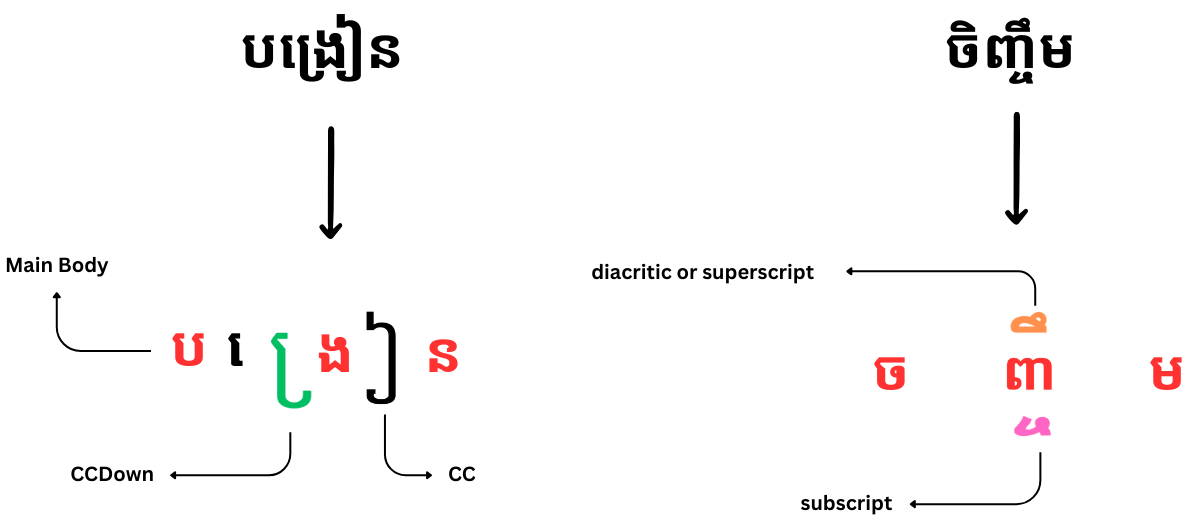
\includegraphics[width=\textwidth]{figures/example_of_text_format.png}
    \caption{Example of Khmer text format showing the complexity of character combinations and diacritics}
    \label{fig:text_format}
\end{figure}

Here's what makes Khmer OCR so different. First, there are no clear word breaks. 
In English, they use spaces between words (it's easy for AI to detect word level). 
Khmer writers use spaces sometimes, sometimes they don't, as you can see in figure
\ref{fig:sequential_text}, so it's really inconsistencies wirting system. This 
makes it impossible to know where one word ends and another begins.

\begin{figure}[H]
    \centering
    
\includegraphics[width=\textwidth]{figures/example_of_long_text.png}
    \caption{Example of sequential Khmer text showing how characters combine to form syllables and words}
    \label{fig:sequential_text}
\end{figure}

A growing challenge in modern Cambodia is the increasing prevalence of mixed-language 
documents that combine Khmer and English text. As English education and international 
business have expanded over the past two decades, it's become common to see documents, 
signs, textbooks, and digital content that seamlessly blend both languages within the 
same sentence or paragraph.

\begin{figure}[H]
    \centering
    
\includegraphics[width=\textwidth]{figures/mix_language_khmer_and_english.png}
    \caption{Example of mixed Khmer-English text showing how both languages appear together in modern Cambodian documents}
    \label{fig:mix_language}
\end{figure}

This mixed-language phenomenon creates several specific problems for OCR systems:
\begin{itemize}
    \item \textbf{Script switching confusion:} OCR models must quickly adapt between completely different writing systems within the same text line
    \item \textbf{Different text layouts:} English flows horizontally while Khmer has vertical stacking, creating complex spatial relationships
    \item \textbf{Font inconsistencies:} The same document often uses different fonts for Khmer and English portions, confusing recognition model
\end{itemize}

Most existing Khmer OCR systems are designed for single-language scenarios 
and perform poorly when encountering this mixed-language reality 
that's everywhere in Cambodia today. Then there's the data problem. To develop high 
accuracy OCR model needs tons of millions annotated images. English has millions 
of labeled images already, How about Khmer lanugage? 
Finding sufficient training data presents a significant challenge. 
While English has millions of labeled training samples, Khmer language 
resources are extremely limited, with only a few thousand quality annotated 
samples available. The situation becomes even more challenging when seeking 
properly labeled mixed-language datasets that combine Khmer and English text. Without enough 
training data, OCR model stays dumb. It can't learn the 
patterns to recognize text accurately.

\begin{figure}[H]
    \centering
    
\includegraphics[width=\textwidth]{figures/varianty_of_font.png}
    \caption{Examples of the same Khmer text rendered in different fonts, demonstrating the significant visual variations that OCR systems must handle}
    \label{fig:font_variants}
\end{figure}

And let's talk about fonts. English has maybe around 15 to 25 common fonts that most people use,
based on reported study use case, from website such as rigorousthemes.com, lifehack.org, and indeed.com. 
Khmer has many different fonts that look very unique from each other, some are thick and bold, others are 
thin and delicate, some have fancy decorations. To train model on one font and 
it fails completely on another.

Look at Figure \ref{fig:font_variants}. Same text, different fonts. To a human, 
it's obviously the same sentence, to a computer, it might be different look.

\begin{figure}[H]
    \centering
    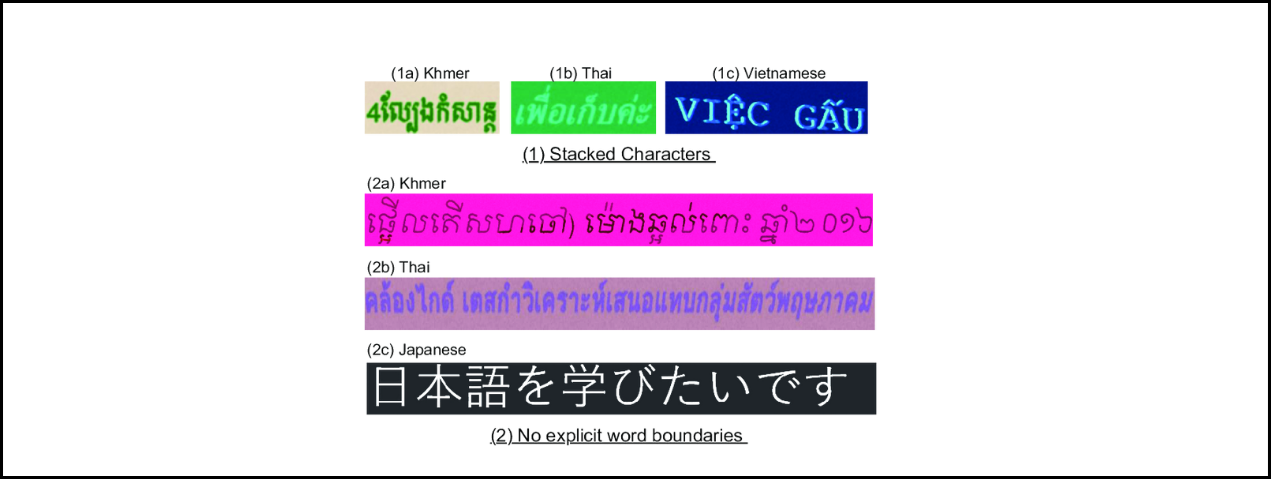
\includegraphics[width=\textwidth]{figures/text_stacking_mixing_language.png}
    \caption{Illustration of Khmer text stacking patterns, 
    showing how characters combine vertically and horizontally 
    to form syllables and words \citep{buoy2023khmerocr}}
    \label{fig:text_stacking}
\end{figure}

That's exactly why we need a better approach. Current OCR tools aren't 
built for the messy reality of Khmer text. They expect perfect conditions
and worked with char-level, word-level only,
that just don't exist in the real world.

\section{Aim and Objectives of the Study}
\label{sec:objectives}

Here's what we're trying to do. We want to build an OCR system that actually 
works for real Khmer documents. Not just clean textbook pages, but the messy, 
mixed-language stuff you see everywhere in Cambodia. Our main goal is simple: 
create an OCR system that can handle both Khmer and 
English text in the same document with high accuracy. Something that doesn't 
fall apart when it sees a content on social media or a textbook page.

To get there, we need to tackle specific problems:

\begin{enumerate}
    \item \textbf{Create a text annotation tool:    } Before we can train anything, we need a way to mark up images with bounding boxes and text labels. We'll build our own tool that can handle both tasks such as text detection and text recognition efficiently.

    \item \textbf{Generate synthetic data that actually helps:} Real data is expensive and time-consuming to collect. We'll create millions of synthetic images that look realistic enough to train our models. Different fonts, various backgrounds, realistic noise and distortions.

    \item \textbf{Build an end-to-end OCR pipeline:} We're using CRAFT for text detection and TrOCR for recognition. But we need to modify them to work well with Khmer script and mixed-language content. This means customizing the models, not just using them out of the box.

    \item \textbf{Make it work in the real world:} Our system needs to handle text lines, not just individual characters. It should work on documents with varying quality, different fonts, and mixed Khmer-English content.

    \item \textbf{Beat existing solutions:} We want to achieve better accuracy than current OCR tools like Tesseract when it comes to Khmer text (excluding commercial models). And we want to do it reliable, not just for testing a few samples.
    
    \item \textbf{Provide an easy-to-use inference model:} Instead of hosting a public API, we’ll share our OCR model on Hugging Face so developers and businesses can run it themselves with minimal setup—no need to dive into technical details. Making the model accessible allows others to test its quality and helps the community continue improving Khmer OCR systems.
\end{enumerate}

The end result should be an OCR system that Cambodian schools, libraries, 
and businesses can actually use. Something that turns physical Khmer documents 
into searchable, editable digital text without requiring a PhD to operate.
That's the goal, Build something that solves real problems for real people.


\section{Research Questions}
\label{sec:questions}

We're trying to answer some pretty fundamental questions about Khmer OCR. Here's what we need to figure out:

\begin{enumerate}
    \item \textbf{Can we make CRAFT and TrOCR work well with Khmer script?} These models were built for English and other Latin languages. Khmer has stacked characters and weird spacing. Will these architectures even work, or do we need to change them completely?

    \item \textbf{How much synthetic data do we actually need?} Everyone talks about generating fake training images, but how many is enough? Can synthetic data really replace real photos of Khmer text? And what kind of augmentation tricks actually help versus just adding noise?

    \item \textbf{What's the minimum dataset size to get decent results?} We don't have Google's budget for data collection. So what's the smallest amount of real annotated data we need to train a working system? Is 1,000 images enough? or 10,000 images? or even more?

    \item \textbf{Can one system handle both Khmer and English effectively?} Mixed language documents are everywhere in Cambodia. But can a single OCR pipeline really switch between two completely different writing systems? Or do we need separate models that somehow work together?

    \item \textbf{What accuracy can we realistically achieve in real conditions?} Lab conditions with clean fonts are one thing. Real documents with blur, shadows, and weird angles are another. What's a realistic target for character error rate on actual Cambodian documents?

    \item \textbf{How do we make this system actually usable?} Building a model that works in Python notebooks is easy. Making something that regular people can use through an API? That's harder. What's the best way to deploy this so it actually helps people?
\end{enumerate}

These questions matter because answering them will tell us whether this whole approach is worth pursuing. And if it works, how to make it work better.

\section{Rationale of the Study}
\label{sec:rationale}
       This research is motivated by several compelling factors. First, there is an urgent need to digitize and preserve Cambodia's vast textual heritage, including historical documents, educational materials, and cultural artifacts. Without effective OCR technology for Khmer script, this digitization process remains labor-intensive and prone to errors.

Second, the current limitations of OCR systems for Khmer significantly hinder educational and academic initiatives in Cambodia. Many educational institutions struggle to convert physical textbooks and learning materials into digital formats, impacting accessibility and modernization efforts in education.

Third, the unique challenges posed by Khmer script—from character stacking to the absence of word boundaries—present an opportunity to advance the field of OCR technology as a whole. Solutions developed for Khmer may benefit other scripts with similar characteristics.

Finally, improving Khmer OCR technology aligns with broader digital transformation goals in Cambodia, supporting efforts to preserve cultural heritage while enabling more efficient information processing and accessibility in various sectors.

\section{Limitations and Scope}
\label{sec:limitations}

While this research aims to advance Khmer OCR technology significantly, it is important to acknowledge certain limitations and define the scope of the study:

\begin{enumerate}
    \item The research focuses specifically on printed Khmer text and English text and does not address handwritten text recognition, which presents additional challenges requiring separate investigation.
    
    \item The study primarily considers modern Khmer fonts and typography, with limited coverage of historical or decorative text styles.
    
    \item While the system aims to handle various document quality levels, extremely degraded or damaged documents may fall outside the scope of reliable recognition.
    
    \item The study focuses on optical character recognition and does not extend to higher-level natural language processing tasks such as semantic analysis or machine translation.
    
    \item Resource constraints may limit the size and diversity of the training dataset, though efforts will be made to ensure sufficient representation of common use cases.
\end{enumerate}

These limitations help maintain a focused research scope while acknowledging areas that may require future investigation.

\section{Structure of the Thesis}
\label{sec:structure}

This thesis is organized into the following chapters:

\begin{enumerate}
    \item \textbf{Introduction}: Presents the research background, objectives, research questions, rationale, and scope of the study.
    
    \item \textbf{Literature Review}: Reviews existing OCR technologies, challenges in Khmer script recognition, and relevant deep learning approaches.
    
    \item \textbf{Methodology}: Details the proposed approach, including dataset preparation, model architecture, and training procedures.
    
    \item \textbf{Implementation}: Describes the technical implementation, including preprocessing techniques, model modifications, and system integration.
    
    \item \textbf{Results and Analysis}: Presents experimental results, performance analysis, and comparative evaluation with existing solutions.
    
    \item \textbf{Conclusion}: Summarizes key findings, contributions, and suggests directions for future research.
\end{enumerate}
Each chapter builds upon the previous ones to present a comprehensive study of Khmer OCR development.

\chapter{Literature Review}
\phantomsection
\label{ch:literature}

\section{Overview}
\phantomsection
\label{sec:ocr-overview}
​ ​ ​ ​ This chapter provides a comprehensive literature review covering several 
key aspects of Optical Character Recognition (OCR). 
It begins with a definition of OCR, followed by an overview of its technological
 evolution over time. Particular attention is given to the unique challenges 
 associated with Khmer OCR, a low-resource language with complex script characteristics.
  The chapter also explores the significant role of synthetic data in addressing data 
  scarcity for low-resource language processing and dataset development.
   Finally, the chapter concludes by identifying and summarizing the existing 
   research gaps in the current literature, highlighting areas that remain 
   under-explored and underscoring the need for further investigation.


\section{Definition of Optical Character Recognition (OCR)}
\phantomsection
\label{sec:ocr-definition}
​ ​ ​ ​ Optical Character Recognition (OCR) is a field of computer vision and pattern recognition
 that focuses on the automatic identification and digitization of printed or handwritten 
 text from images, scanned documents, or other visual media \citep{singh2012survey}. 
 OCR systems aim to convert visual representations of text into machine-encoded formats, 
 enabling automated indexing, editing, and data extraction \citep{muaz2015khmerocr}.

Modern OCR technology has evolved significantly from its early rule-based and template-matching
roots to incorporate advanced machine learning techniques, particularly deep learning,
which allow for improved accuracy in character detection, segmentation, and classification across 
diverse languages and scripts.

OCR systems typically consist of several key components: image preprocessing (e.g., noise removal, binarization), text detection, character segmentation, feature extraction, and recognition. These systems must be adapted to handle various font styles, image distortions, complex layouts, and script-specific features. While OCR for Latin-based languages has become highly accurate, extending such systems to non-Latin scripts—such as Khmer—remains a significant research challenge due to unique linguistic and structural characteristics.
  

\section{Text Detection}
\phantomsection
\label{sec:text_detection_literature}

  ​ ​ ​ ​  \citet{Hiremath_text_detection} The task of detecting text regions in images is a 
crucial first step in many document analysis pipelines.Character Region Awareness by \citet{Baek}
proposed an efficientand accurate scene text detection approach by incorporating character region 
masking and attention. 

\citet{Hiremath_text_detection} Some other popular research Methodology for text detection and 
highly cited text detection algorithms such as:

EAST (Efficient and Accurate Scene Text Detector) \citet{Zhou} uses a fully convolutionalnetwork to 
directly predict word or text line bounding boxes along with their orientation. 
It was one of the first modern deep learning models for this task. TextBoxes++ \citet{TextBoxes}
extended the TextBoxes model with more powerful convolutional features and anangle 
vector to better handle oriented and curved text instances.  CRAFT (CharacterRegion Awareness for 
Text Detection) \citet{Baek} akes a different approach, using a regionscore map to localize 
individual character regions which are then grouped into words/text lines.
Mask TextSpotter \citet{TextSpotter} combines semantic segmentation + attention-based 
recognition to directly read text of any shape from natural scenes—all in one unified model.
TextFuseNet \citet{ijcai2020p72} is detects text by extracting and fusing features 
at three levels: character-level, word-level, and global-level. It uses a semantic segmentation 
branch for global context, detects characters and words through a modified Mask R-CNN pipeline, 
and combines all levels using a multi-path fusion architecture. This fusion enriches the text 
representation, enabling the model to better localize and segment text instances of arbitrary shapes.
ABCNet \citet{ABCNet} have been proposed which aim to jointly optimize text detection and 
recognition in a unified architecture. Such unified frameworks potentially allow the two tasks 
to benefit from each other during training. 

% Define a custom column type for better control
\newcolumntype{L}[1]{>{\raggedright\arraybackslash}p{#1}} % left-aligned fixed width
\newcolumntype{C}[1]{>{\centering\arraybackslash}p{#1}}   % centered fixed width

\begin{table}[H]
  \centering
  \caption{Text Detection Accuracy}
  \begin{tabularx}{\linewidth}{|L{3.5cm}|L{2.5cm}|L{2.5cm}|C{2cm}|C{2cm}|C{2cm}|}
    \hline
    \textbf{Model} & \textbf{Backbone} & \textbf{Dataset} & \textbf{Recall (\%)} & \textbf{Precision (\%)} & \textbf{F1-score (\%)} \\
    \hline
    EAST* & VGG-16 & ICDAR 2015 & 78.3 & 83.3 & 80.7 \\
    He et al. & ResNet-50 & ICDAR 2015 & 80.0 & 82.0 & 81.0 \\
    R2CNN & VGG-16 & ICDAR 2015 & 79.7 & 85.6 & 82.5 \\
    TextSnake & VGG-16 & ICDAR 2015 & 80.4 & 84.9 & 82.6 \\
    TextBoxes++* & VGG-16 & ICDAR 2015 & 78.5 & 87.8 & 82.9 \\
    EAA & ResNet-50 & ICDAR 2015 & 83.0 & 84.0 & 83.0 \\
    Mask TextSpotter & ResNet-50 & ICDAR 2017 & 81.2 & 85.8 & 83.4 \\
    PixelLink* & VGG-16 & ICDAR 2017 & 82.0 & 85.5 & 83.7 \\
    RRD* & ResNet-50 & ICDAR 2017 & 80.0 & 88.0 & 83.8 \\
    Lyu et al.* & ResNet-50 & ICDAR 2017 & 79.7 & 89.5 & 84.3 \\
    FOTS & ResNet-50 & ICDAR 2017 & 82.0 & 88.8 & 85.3 \\
    CRAFT & VGG-16 & ICDAR 2015 & 84.3 & 89.8 & 86.9 \\
    \hline
  \end{tabularx}
  \caption*{Source: Results sourced from the CRAFT research paper \cite{Hiremath_text_detection}. 
  Results are reported on quadrilateral-type datasets such as ICDAR. 
  Asterisks (*) denote results based on multi-scale tests. 
  The table compares various scene text detection models—including the CRAFT model used in the proposed system—across key performance metrics such as precision, recall, and F1-score.}
  \label{tab:text_detection_accuracy}
\end{table}

\vspace{1em}



\section{Khmer Optical Character Recognition (OCR)}
\phantomsection
\label{sec:khmer_OCR_literature}

​ ​ ​ ​ \citet{CheyFirstOCR} The first significant research on Optical Character Recognition (OCR) 
for Khmer script was proposed in 2006, marking a foundational contribution 
to Khmer language digitization. The study addressed critical challenges 
inherent to Khmer printed characters, notably the variation in character 
shapes across fonts and the high visual similarity between certain 
characters. To overcome these issues, the authors introduced a novel 
recognition method utilizing Wavelet Descriptors. The approach involved 
transforming printed character images into their skeleton forms, 
then converting these skeletons into the temporal domain. Character 
templates were generated using wavelet coefficients from a training set, 
and recognition was performed through a deformable wavelet descriptor 
and a Euclidean distance classifier. The recognition process selected 
the template with the smallest distance to the input character as the 
result. Interestingly, deformation was later excluded from the final 
method due to its adverse impact on distinguishing similar characters. 
Experimental evaluation demonstrated promising results: recognition 
rates of 92.85\%, 91.66\%, and 89.27\% for 22-point, 18-point, and 
12-point font sizes respectively, across 10 Khmer fonts. A second 
test used a 21-page document scanned at varying resolutions 
(150, 300, 600 dpi) and fax inputs, achieving recognition rates 
of 92.99\% at 300 dpi, 88.61\% at 150 dpi, and 80.05\% for faxed documents. 
This pioneering work laid the groundwork for future Khmer OCR systems 
and remains a landmark study in Khmer script recognition.

\citet{Sok&Taing2014} The second significant research on 
Khmer Optical Character Recognition (OCR) introduces a Support 
Vector Machine (SVM)-based approach for printed Khmer character 
recognition in bitmap documents. Given the inherent complexity 
of the Khmer script—which includes 74 alphabets and the potential 
for up to five vertical levels in word compounds—the study focuses 
on identifying the most effective SVM kernel for classification.

The proposed method evaluates three SVM kernels: Gaussian, Polynomial, 
and Linear. Rather than training on large datasets, the system adopts 
a modular approach, segmenting characters into smaller parts. Each 
segment is transformed into a binary matrix, with 1s representing 
black pixels and 0s for whitespace. Feature extraction is applied 
to these matrices for SVM training and classification.

Following recognition, post-processing rules are employed to merge 
character clusters and correct common misclassifications based on 
character levels. The training utilized one font ("Khmer OS Content") 
at 32pt and tested recognition performance across three font sizes 
(28pt, 32pt, and 36pt). The results demonstrated strong accuracy:
\begin{itemize}
  \item 98.17\% for 28pt,
  \item 98.62\% for 32pt,
  \item 98.54\% for 36pt.
\end{itemize}

The Gaussian kernel outperformed the other kernels, confirming its 
suitability for Khmer character recognition. This study highlights 
the effectiveness of machine learning-based OCR for complex scripts 
like Khmer and marks a major advancement over earlier template-based 
systems.

\citet{Meng_Hann_2014} proposed a Khmer Character Recognition (KCR) 
system utilizing artificial neural networks to address the complexity 
of recognizing individual Khmer script characters. Developed in a 
MATLAB environment, the system integrates a Self-Organizing Map (SOM) 
for unsupervised clustering with a Multilayer Perceptron (MLP) 
trained via the backpropagation algorithm for supervised classification. 
The recognition process follows a two-stage pipeline: first, the input 
image—resized to 20×20 pixels—is categorized by the SOM into one of 
nine coarse groups. Then, each group is assigned to a dedicated MLP 
model, which performs fine-grained classification into one of 82 
target classes, including Khmer consonants, vowels, and numerals. 
This modular approach aims to enhance classification efficiency by 
narrowing the decision space for each MLP. The system achieved an 
average recognition accuracy of 65\% on the training dataset and 
30\% on the testing dataset, highlighting both the potential and 
the challenges of neural network-based Khmer OCR at the time.

\citet{Muaz2015} This study presents a comprehensive OCR system for 
printed Khmer text using the HTK Toolkit, covering the full 
pipeline of pre-processing, segmentation, recognition, and mapping. 
The system is tailored for the widely used Limon S1 font at 22pt and 
introduces a structural segmentation approach that decomposes 
characters into five categories: Main Body, SuperScript, SubScript, 
CCDown, and Complex Character (CC). Feature extraction relies on 
vertical framing and Discrete Cosine Transform (DCT), with 
classification handled by Hidden Markov Models (HMMs). 
The system was trained on over 35,000 labeled shape samples and 
evaluated on 10 pages of scanned newspaper text, achieving an 
overall recognition rate of 96.34\%. While the results are promising, 
the system is limited by its reliance on a single font style and size, 
making it less robust to font variation. Additionally, recognition 
performance drops for complex shapes like CC (70.88\%) and depends 
heavily on manually crafted mismatch and rule files for post-processing, 
indicating scalability and generalization challenges for real-world 
applications involving diverse document types and fonts.

\citet{Valy_8563219} proposed a character-level Convolutional Neural 
Network (CNN) model for recognizing ancient Khmer script from digitized 
palm leaf manuscripts. The study focuses on two core tasks: 
isolated character recognition and word-level glyph localization. 
For the character recognition task, a CNN architecture comprising 
three convolutional blocks followed by a linear classifier was 
developed. The output layer of the network predicts one of 106 
character classes, achieving a reported test accuracy of 95.96\%. 
In addition to CNNs, the study also explores other neural 
architectures including LSTM-RNN and hybrid CNN-RNN models. 
For the word/text image recognition task, the authors leveraged 
both one-dimensional and two-dimensional RNNs to handle the complex 
spatial structure of Khmer script and to localize glyphs within 
variable-length text patches. This research highlights the potential 
of deep learning approaches in historical Khmer OCR, particularly in 
handling the challenges posed by degraded manuscripts and complex 
writing structures.

\citet{Annanurov_2018} conducted a pilot study on Khmer handwritten 
symbol recognition, focusing on the use of Convolutional Neural 
Networks (CNNs) for digitizing large-scale handwritten document corpora. 
The study used image data from six handwriting datasets containing 
33 Khmer consonants and 17 vowels, forming a total of 561 syllables. 
For consonant recognition, the authors trained 33 individual CNNs—one 
for each root radical—which were later integrated into a recognition 
assembly. The performance of the CNN-based model was evaluated against 
two alternative systems: an artificial neural network (ANN) using the 
full feature set, and another ANN with reduced feature dimensions. 
Feature extraction techniques such as two-dimensional Fourier 
transformation (FT2D) and Gabor filters were employed for dimensionality 
reduction. The CNN-based approach achieved a recognition accuracy of 
up to 94.85\%, outperforming the ANN-based models. However, the system 
was limited to recognizing only Khmer consonants, without support for 
vowel or syllable-level recognition.

\citet{sokphyrum2019khmer} fine-tuned the Tesseract OCR engine 
(version 4.0) to improve recognition of Khmer Unicode and legacy 
Limon fonts. Tesseract 4.0 employs a deep convolutional recurrent 
neural network with a connectionist temporal classification (CTC) 
loss function and attention mechanism, enabling it to recognize entire 
text-line images. The fine-tuning process involved training on 14 Khmer 
Unicode fonts and 20 pre-Unicode Limon fonts (all at 12pt size). 
The ISRI Analytic Tools were used to evaluate OCR accuracy at both 
the character level (CHL) and cluster level (CLL) by comparing OCR 
outputs to ground truth text. The Khmer pre-trained engine achieved 
an average accuracy of 87.49\% at the character level and 89.43\% at 
the cluster level on Unicode fonts, while legacy Limon fonts yielded 
a significantly lower median accuracy of 62.27\%. After fine-tuning, 
recognition accuracy reached up to 90\% for specific fonts, demonstrating 
the potential of domain-specific adaptation to enhance OCR performance 
for complex scripts like Khmer.


\citet{Buoy2022} Khmer printed character recognition presents significant 
challenges due to the script's complex structure, including stacked consonants, 
dependent vowels, and diacritics placed in various positions. Traditional approaches, 
such as SVMs, wavelet-based templates, and CNNs, have largely focused on recognizing standalone 
characters and depend heavily on accurate segmentation, making them less robust for noisy or 
continuous text-line images. Tesseract OCR, though improved with deep neural networks 
and CTC loss, still performs poorly on heavily augmented images with a reported Character 
Error Rate (CER) of 35.9\%. In contrast, the reviewed study introduces an end-to-end 
attention-based Sequence-to-Sequence (Seq2Seq) model that directly maps entire text-line 
images to character sequences without needing pre- or post-processing. Trained on 3 million 
synthetically generated and augmented images across multiple Khmer fonts, the model 
achieved a CER of 0.7\% on noisy images and 0.24\% on clean images, significantly 
outperforming existing methods and demonstrating the effectiveness of attention mechanisms 
and deep learning for low-resource scripts like Khmer.

\citet{nom2024khmerst} The Khmer script poses significant challenges for scene text detection 
and recognition due to its complex structure involving stacked consonants, multiple diacritics, 
subscript characters, and the lack of explicit word boundaries. To address the scarcity of 
resources for this low-resource language, this study introduces KhmerST, the first annotated 
scene-text dataset for the Khmer language, consisting of 1,544 real-world images captured 
from various public settings in Cambodia. Unlike existing synthetic Khmer datasets, 
KhmerST includes indoor and outdoor images with diverse fonts, orientations, and 
background conditions, and provides polygon-based line-level annotations for more accurate 
localization. Benchmarking with YOLO models shows that YOLOv8 performs best in detection 
tasks due to its ability to handle small and variable text elements, while in recognition 
tasks, both TrOCR and Tesseract perform poorly, with TrOCR achieving CER of 0.90 and 
Tesseract CER of 1.30, highlighting the need for Khmer-specific OCR models. The study 
underscores the gap between current OCR systems and the needs of Khmer script recognition, 
calling for future research on synthetic data generation, Khmer-aware model design, 
and multimodal approaches to improve accuracy in real-world applications.

\citet{Rina2025} This research addresses the challenge of Khmer textline recognition, 
which is particularly difficult due to the absence of spaces between words in the Khmer script. 
Unlike Latin-based languages, this structure requires recognition to be performed at the textline level, 
leading to high latency when using autoregressive (AR) decoders that predict one character at a 
time while considering previous characters. In contrast, non-autoregressive (NAR) decoders can decode 
all characters in parallel but lack awareness of character dependencies, resulting in lower linguistic 
accuracy. To solve this, the authors propose an efficient Khmer textline recognition method using an NAR 
decoder, enhanced by Khmer-specific subword modeling. Instead of predicting single characters, the model 
recognizes character clusters (subwords), capturing the syntactic, morphological, and orthographic 
structure of the language implicitly. This design retains the speed of NAR models while improving accuracy. 
Experimental results show that the proposed method outperforms the character-level NAR baseline 
in accuracy and matches or exceeds the AR baseline while maintaining lower latency. However, 
the abstract does not report detailed accuracy or metrics, and access to full experimental results 
requires a subscription, limiting transparency for non-subscribers. This work contributes an 
important step toward faster and more linguistically aware Khmer OCR by bridging the gap between 
speed and accuracy in scene text recognition.

Khmer OCR research has progressed significantly, yet the script’s structural complexity—including 
stacked consonants, subscript forms, diacritics, and the absence of spaces between words—continues 
to pose major challenges. Early methods relying on wavelet descriptors, SVMs, and HMMs showed moderate 
success but struggled with font variations, segmentation, and real-world noise. Deep learning has 
since enabled end-to-end approaches like attention-based Sequence-to-Sequence (Seq2Seq) models, 
achieving state-of-the-art accuracy with character error rates (CER) as low as 0.24\% on clean 
images and 0.7\% on noisy inputs. However, general-purpose engines like Tesseract still perform 
poorly, especially in scene text scenarios, as highlighted by results from the newly introduced 
KhmerST dataset. A promising direction involves non-autoregressive (NAR) models enhanced with 
Khmer-specific subword modeling, which offer faster inference and comparable or better accuracy 
than autoregressive (AR) models. Despite these advances, many studies lack open access to detailed 
results, and gaps remain in handwritten recognition, font diversity, and domain adaptation. 
Future research must prioritize Khmer-aware model design, synthetic data generation, and robust 
multimodal solutions to improve performance in real-world OCR applications.
    
\begin{figure}[ht]
    \centering
    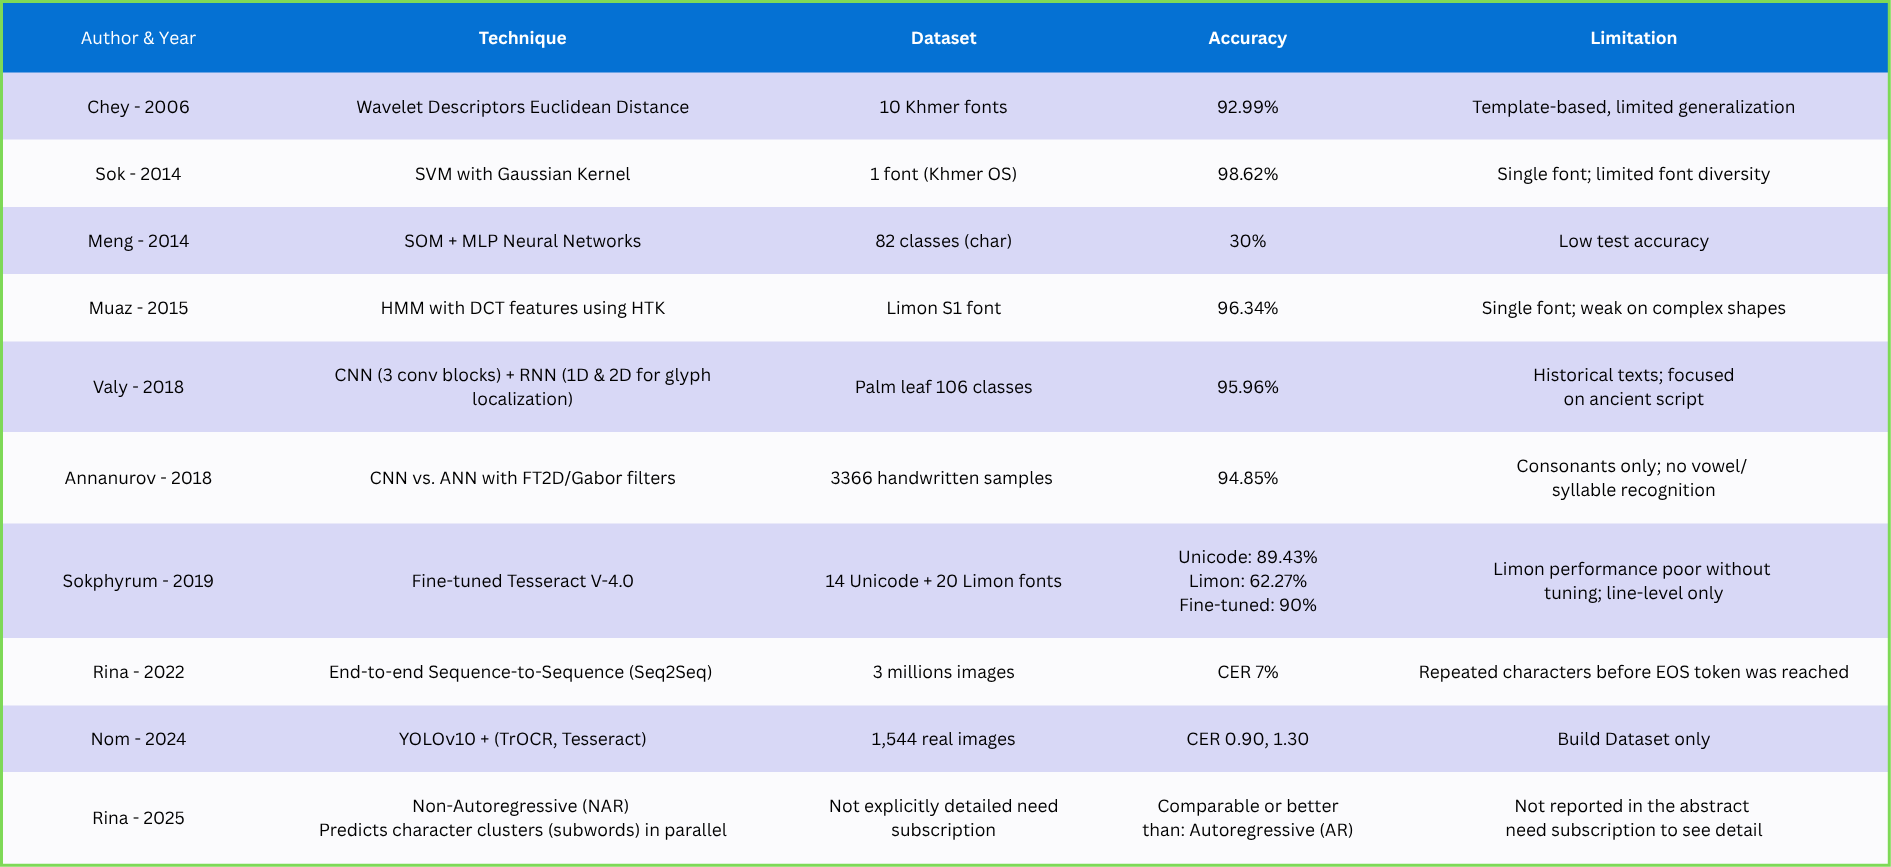
\includegraphics[width=\textwidth]{figures/summary_literature_review.png}
    \caption{Summary of the literature review, which includes the types of models used, 
    the datasets used, the metrics used to evaluate the performance of the models, 
    and the results of the experiments. The table highlights the key findings of the 
    literature review, including the challenges faced when developing Khmer OCR models 
    and the need for Khmer-specific models and datasets.}
    \label{fig:summary_literature_review}
\end{figure}

\section{Challenges in Khmer OCR}
\phantomsection
\label{sec:datasets}

Khmer OCR poses numerous technical challenges stemming from the script's unique structure and 
linguistic features. Unlike Latin-based scripts, Khmer characters can include complex stacking 
of consonants (e.g., subscript consonants using Coeng), placement of diacritics, and variable vowel 
positions that appear above, below, before, after, or even wrap around base characters \citep{buoy2021seq2seq}. 
This spatial complexity makes segmentation particularly difficult and often unreliable, 
especially in cluttered or noisy environments. Accurate character separation is further complicated 
by the fact that multiple elements can visually overlap, causing traditional segmentation-based 
approaches to fail.

Font diversity also adds a layer of complexity. Khmer is written using a wide array of fonts, each 
introducing variations in stroke thickness, character proportions, and spacing. These stylistic 
differences can drastically alter a character's appearance, requiring OCR systems to be highly 
font-invariant \citep{buoy2021seq2seq}. Yet, many models are trained on limited font sets, leading 
to poor generalization across unseen styles.

Another critical issue is the scarcity of annotated datasets. As a low-resource language, Khmer lacks 
the extensive labeled corpora available for Latin or Chinese scripts. This data scarcity hampers the 
training of robust models and forces researchers to rely on synthetic data or heavily augmented datasets 
to simulate real-world variability.

Additionally, many legacy OCR systems for Khmer rely on rule-based or modular pipelines with explicit 
character segmentation, manual pre- and post-processing, and assumptions about text structure. These 
approaches are brittle and poorly suited for real-world applications where scanned documents may contain 
noise, skew, blur, uneven lighting, or distorted text lines. Their reliance on handcrafted rules also 
limits scalability and adaptability to other domains.

Lastly, the lack of word boundaries in Khmer—where text is often written without spaces—presents an 
additional recognition barrier. This linguistic feature necessitates full line-level recognition, 
which increases computational complexity and requires models to understand broader contextual dependencies 
across characters.



\section{Role of Synthetic Data}
\phantomsection
\label{sec:dl-models}

To overcome the challenges associated with data scarcity in Khmer OCR, 
recent studies have emphasized the critical role of synthetic data generation. A prominent 
strategy involves leveraging the open-source \texttt{text2image} utility from the Tesseract OCR 
engine to create high-quality, rendered images of Khmer text lines \citep{buoy2021seq2seq}. 
These images are generated from a curated text corpus that includes a diverse mix of numbers, 
words, phrases, and full sentences, providing broad linguistic coverage.

Multiple commonly used Khmer fonts are applied during rendering to simulate font diversity and 
improve the model's ability to generalize across different typographic styles. Each rendered 
image is converted to grayscale and resized to a fixed height (e.g., 32 pixels) to meet the input 
dimensional requirements of neural network models, while maintaining proportional width to preserve 
text structure.

To emulate real-world conditions and enhance robustness, extensive data augmentation techniques 
are applied. These include Gaussian blurring, morphological operations like dilation and erosion, 
speckle and blob noise injection, background texture overlays, rotational distortions, and random 
concatenation of multiple text-line images. Each augmentation has a 50\% probability of being applied, 
with combinations occurring dynamically during training to maximize variability and minimize overfitting.

The resulting synthetic dataset scales to millions of samples, covering a wide spectrum of distortions, 
font styles, and text structures. This scale and diversity enable deep learning models—particularly 
end-to-end architectures such as attention-based Sequence-to-Sequence networks—to learn robust 
visual and contextual features, improving performance on both clean and noisy inputs. Ultimately, 
synthetic data serves as a vital resource for building Khmer OCR systems capable of handling the 
script’s inherent complexity in the absence of large, annotated real-world datasets.


\section{Summary of Research Gaps}
\phantomsection
\label{sec:research-gaps}

Despite recent progress in Khmer Optical Character Recognition (OCR), 
several critical gaps persist in the current body of research, hindering the 
development of robust and generalizable systems. First and foremost is the issue of 
data scarcity—there is a lack of large-scale, high-quality annotated datasets for Khmer, 
particularly for scene text and handwriting, which restricts model training, benchmarking, 
and cross-domain evaluation. Although synthetic datasets have partially mitigated this, they 
cannot fully replicate the variability and unpredictability of real-world documents. Second, the 
complex structural features of Khmer script—such as stacked consonants, overlapping vowel markers, and 
the absence of explicit word boundaries—are insufficiently addressed in many existing models, 
especially those adapted from Latin-script OCR frameworks. These models often fail to 
capture the script's spatial dependencies and morphological nuances. Third, font 
variability remains a major bottleneck: Khmer documents are written in a wide range of stylistic 
fonts, and OCR systems trained on limited font sets often generalize poorly. Lastly, there is 
a lack of robustness to real-world document conditions, including noisy backgrounds, image blur, 
skew, and low resolution. Many current systems, including Tesseract and some CNN-based models, 
show significant performance drops under such conditions. Addressing these gaps—through 
Khmer-specific model design, comprehensive dataset creation, and more resilient training strategies—is 
essential for building high-performance OCR systems tailored to the Khmer language and its 
real-world use cases.

\chapter{Dataset Construction}
\phantomsection
\label{ch:dataset}

\section{Text Source Collection}
\label{sec:text-source}
This section describes the process of collecting Khmer text data from various sources to create a comprehensive dataset for OCR training and evaluation.

\subsection{Khmer Websites and Dictionaries}
\label{subsec:websites}
We gathered text samples from popular Khmer news websites, online dictionaries, and digital libraries to ensure diverse vocabulary coverage and writing styles.

\subsection{Online NLP Resources and Tools} 
\label{subsec:nlp-tools}
Additional text data was collected using available Khmer NLP tools and resources, including pre-existing corpora and language processing utilities.

\section{Text Cleaning and Preprocessing}
\label{sec:preprocessing}
Raw text data underwent several preprocessing steps to ensure quality and consistency for synthetic image generation.

\subsection{Removal of Invalid Characters and Whitespace}
\label{subsec:cleaning}
We implemented filtering mechanisms to remove invalid Unicode characters, normalize whitespace, and handle special characters that could affect OCR performance.

\subsection{Unicode Normalization}
\label{subsec:unicode}
All text was normalized to ensure consistent Unicode representation of Khmer characters and their combinations.

\section{Sentence Segmentation and Reconstruction}
\label{sec:segmentation}
The cleaned text was processed to create meaningful sentence units suitable for OCR training.

\subsection{Tokenization Using khmer-nltk}
\label{subsec:tokenization}
We utilized the khmer-nltk library to perform accurate tokenization of Khmer text while preserving linguistic properties.

\subsection{Sentence Length Variation}
\label{subsec:length}
Sentences were segmented and reconstructed to create samples with varying lengths, ensuring the dataset represents real-world text diversity.

\section{Image Generation Pipeline}
\label{sec:generation}
A robust pipeline was developed to convert processed text into synthetic training images.

\subsection{Font and Background Selection}
\label{subsec:fonts}
Multiple Khmer fonts and background variations were incorporated to create diverse and realistic training samples.

\subsection{Noise Injection Techniques}
\label{subsec:noise}
Various types of noise and distortions were systematically added to simulate real-world document conditions.

\subsection{Image Rotation and Margin Augmentation}
\label{subsec:augmentation}
Geometric transformations and margin variations were applied to improve model robustness to different text orientations and layouts.

\section{Dataset Statistics and Format}
\label{sec:statistics}
This section presents detailed statistics about the generated dataset, including size, character distribution, and format specifications.

\section{Comparison with Existing Datasets}
\label{sec:comparison}
A comparative analysis of our dataset with existing Khmer OCR datasets, highlighting improvements and unique characteristics.

\chapter{Model Architecture and Experiments}
\phantomsection
\label{ch:experiments}

\section{Experimental Environment and Tools}
\label{sec:environment}
All experiments in this study were conducted on a high-performance workstation running 
Ubuntu 20.04 LTS. The system was equipped with dual NVIDIA RTX 4090 GPUs, each with 
48 GB of VRAM, and 128 GB of system RAM, ensuring ample memory and computational power 
for training large-scale deep learning models efficiently.

The models were implemented using the PyTorch deep learning framework, with integration of the Hugging Face Transformers library for state-of-the-art model architectures such as TrOCR. GPU acceleration was enabled via CUDA, allowing for fast and parallelized training across the two GPUs.

For experiment tracking and metric logging, MLflow was used. It captured key training 
and evaluation metrics such as character error rate (CER), word error rate (WER), 
training loss, and validation loss in real-time. This facilitated better experiment 
management and reproducibility, especially when comparing multiple model versions or 
hyperparameter configurations.



\section{Model Architecture and Configuration}
\label{sec:architecture}
Details of the model architectures and configurations used in the OCR system.

\subsection{CRAFT for Text Detection}
\label{subsec:craft}

For the text detection stage, we adopted the Character Region Awareness for Text 
Detection (CRAFT) model, which is well-regarded for its ability to detect text at 
the character level rather than relying solely on word-level bounding boxes. 
CRAFT produces dense predictions of character regions and affinity scores, 
enabling it to localize irregular and closely spaced text lines—an essential 
requirement for handling complex scripts like Khmer.

The CRAFT model architecture consists of a VGG16-based backbone followed by a series 
of convolutional layers to produce two output maps:
\begin{itemize}
\item A \textbf{region score map}, indicating the likelihood of each pixel belonging 
to a character region.
\item An \textbf{affinity score map}, capturing the spatial relationships between 
adjacent characters to form text lines.
\end{itemize}

In this study, we fine-tuned a pretrained CRAFT model on a custom Khmer dataset 
composed of synthetic and real-world scene text images. We applied data augmentation 
techniques such as rotation, scaling, blurring, and illumination changes to increase 
the model's robustness. The input images were resized to a fixed height of 768 pixels 
while preserving the aspect ratio.

We used the official implementation of CRAFT with some modifications to better support
Khmer character characteristics, such as tight spacing, stacked glyphs, and diacritic 
marks. The model was trained using Adam optimizer with a learning rate of 1e-4 and batch 
size of 16. Early stopping and validation-based checkpointing were employed to 
prevent overfitting.

The output of the CRAFT detector was then passed to the text recognition 
model (TrOCR), enabling a two-stage pipeline for accurate and end-to-end 
Khmer text reading in natural scenes.

\begin{figure}[ht]
    \centering
    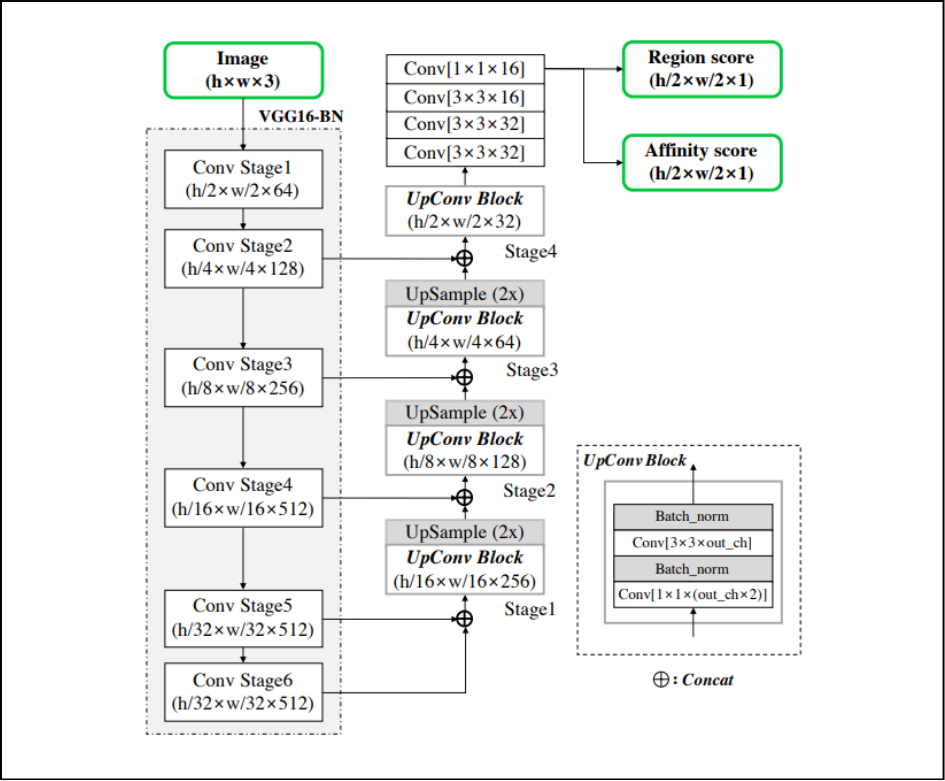
\includegraphics[width=\textwidth]{figures/craft_model.png}
    \caption{Illustration of the CRAFT model architecture used for text detection. \cite{baek2019craft}}
    \label{fig:craft-model}
\end{figure}


\subsection{TrOCR for Text Recognition}
\label{subsec:trocr}

For the text recognition component of the pipeline, we used the \textbf{TrOCR} model, 
a transformer-based OCR system proposed by Microsoft Research. TrOCR stands for 
\textit{Transformer-based Optical Character Recognition}, and it integrates a vision 
encoder with a language decoder in a unified encoder-decoder (Seq2Seq) architecture, 
following the structure of the Vision Transformer (ViT) and pre-trained language models 
like BART.

The TrOCR model takes the cropped text-line image detected by CRAFT and processes it through a \textbf{ViT-based encoder}, which extracts rich visual features. These features are then passed to the \textbf{transformer decoder}, which generates the text sequence token-by-token, using cross-attention to focus on relevant image features while decoding. This allows the model to handle complex scripts like Khmer with better accuracy and context-awareness.

We fine-tuned the base version of TrOCR using the Hugging Face \texttt{transformers} library on our custom synthetic Khmer dataset. During training, we tracked key metrics such as Character Error Rate (CER) and Word Error Rate (WER) using MLflow. The model demonstrated strong generalization across different fonts and text conditions, benefiting from both large-scale pretraining and our domain-specific fine-tuning.

\begin{figure}[ht]
    \centering
    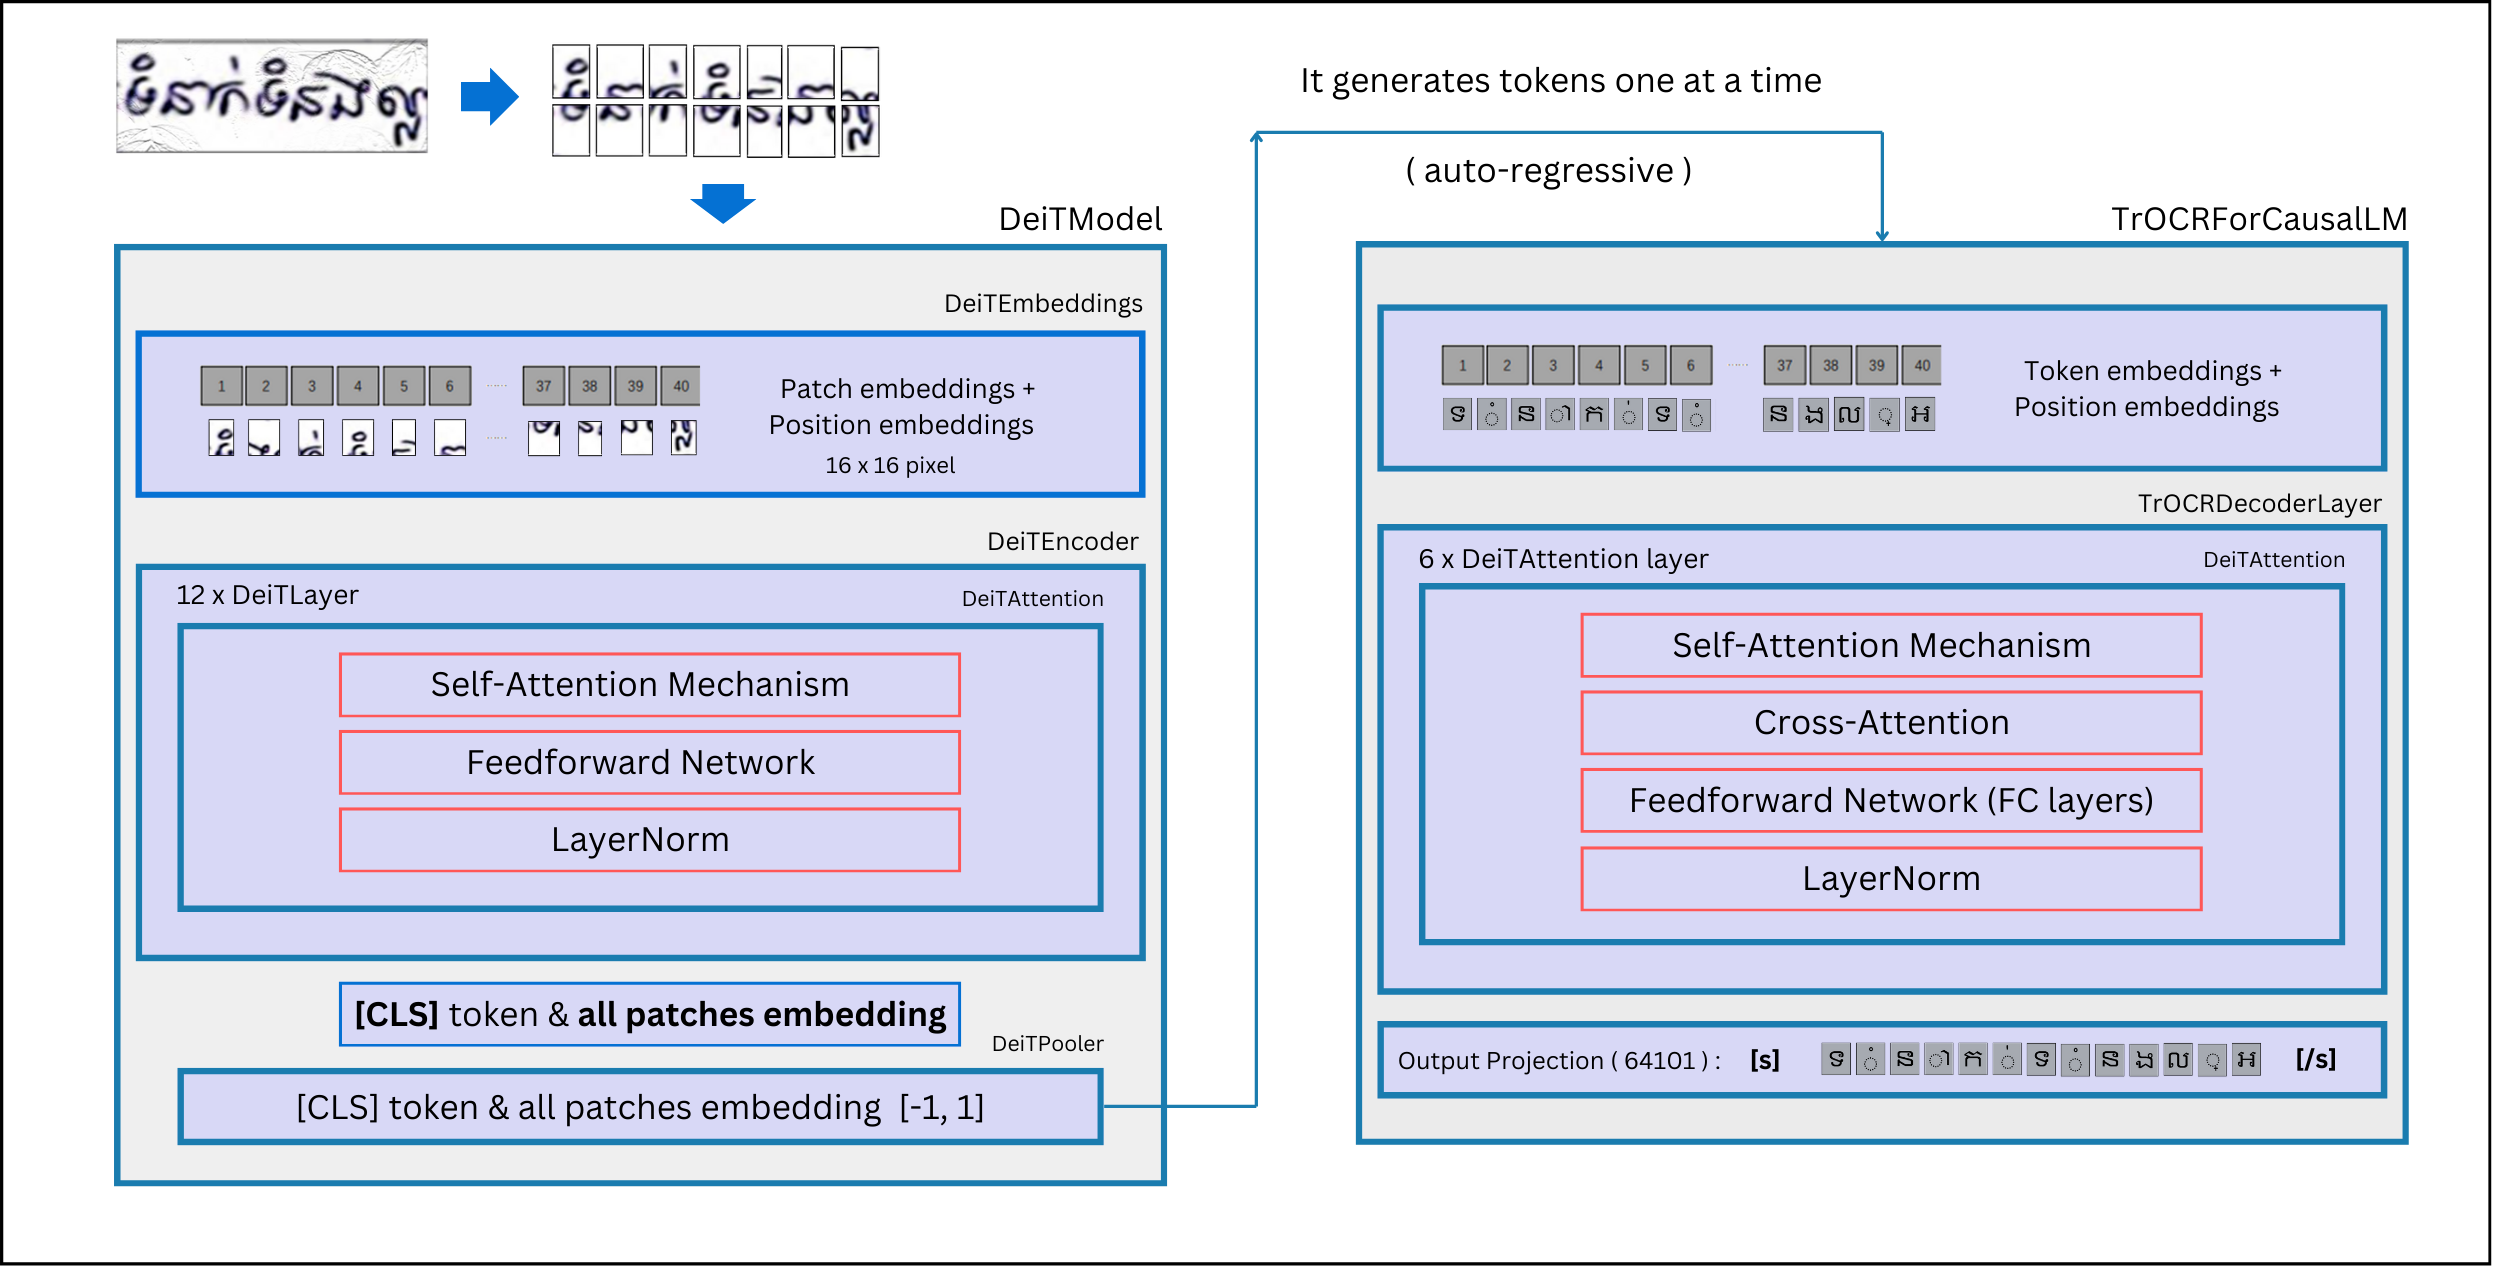
\includegraphics[width=\textwidth]{figures/trocr_model.png}
    \caption{Illustration of the TrOCR model architecture used for text recognition.}
    \label{fig:trocr-model}
\end{figure}


\section{Training Methodology}
\label{sec:training}
This section delves into the training strategies and processes employed to optimize 
the performance and accuracy of the OCR models. We describe the fine-tuning procedures 
for both the CRAFT text detector and TrOCR text recognizer, as well as the key 
hyperparameters and metrics used to evaluate their performance. Additionally, we 
present a discussion on the importance of robust training and the approaches taken 
to ensure the models generalize well across different fonts, text conditions, and 
domains.



\subsection{Fine-tuning Configuration for CRAFT}
\label{subsec:craft-training}

The CRAFT model was fine-tuned on a custom Khmer text dataset using weak supervision, 
leveraging the strengths of annotated real images. During 
training, we applied a range of augmentations to improve robustness against font 
variations, noise, and other distortions. To further enhance the model's generalization 
abilities, we employed techniques such as random cropping, flipping, and rotation to 
increase the diversity of the training data. Additionally, we used a combination of 
contrastive learning and adversarial training to improve the model's ability to 
discriminate between different characters and fonts. Finally, we used transfer learning 
to adapt the model to the Khmer language by fine-tuning it on a small dataset of 4000 
manually annotated bounding boxes. This dataset was carefully curated to capture the 
unique characteristics of the Khmer script, such as its complex diacritic marks and 
ligatures. The most important configuration values for training the CRAFT model are 
summarized in Table~\ref{tab:craft-training-config}, including the training mode, 
backbone architecture, pre-trained weights, loss function, normalization parameters, 
and optimization hyperparameters. These settings are crucial for achieving optimal 
performance on the Khmer text dataset.

\noindent
\textbf{Data Augmentation:} During training, the following augmentations were applied:
\begin{itemize}
    \item \textbf{Random rotation:} Up to 20° (enabled).
    \item \textbf{Random cropping:} Variable scale and aspect ratio.
    \item \textbf{Horizontal flipping:} Enabled.
    \item \textbf{Color jittering:} Adjustments in brightness, contrast, saturation, and hue (each set to 0.2).
\end{itemize}



\begin{table}[ht]
\centering
\begin{tabular}{|p{0.4\linewidth}|p{0.55\linewidth}|}
\hline
\textbf{Parameter} & \textbf{Value} \\
\hline
Training mode & \texttt{weak\_supervision} \\
Backbone architecture & VGG \\
Use of SynthText & False \\ 
Real dataset & \texttt{custom} \\
Pretrained weights & \texttt{CRAFT.pth} \\
Batch size & 5 \\
Training iterations & 0 to 10,000 \\
Evaluation interval & Every 500 iterations \\
Learning rate & 0.0001 \\
Learning rate decay step & 7,500 \\
Decay rate ($\gamma$) & 0.2 \\
Weight decay & 0.00001 \\
Mixed precision (AMP) & Enabled \\
Loss function type & 2 \\
Negative ratio & 0.3 \\
Minimum negative samples & 5,000 \\
Output image size & 768 \\
Normalization mean & [0.485, 0.456, 0.406] \\
Normalization std (variance) & [0.229, 0.224, 0.225] \\
Region enlargement factor & [0.5, 0.5] \\
Affinity enlargement factor & [0.5, 0.5] \\
Gaussian kernel init size & 200 \\
Gaussian sigma & 40 \\
\hline
\end{tabular}
\caption{Key configuration parameters for training the CRAFT model on a custom Khmer dataset 
using weak supervision. The parameters include the training mode, backbone architecture, 
dataset, batch size, training iterations, evaluation interval, learning rate, learning rate decay, 
weight decay, mixed precision, loss function type, negative ratio, minimum negative samples, 
output image size, normalization mean and standard deviation, region and affinity enlargement 
factors, Gaussian kernel initialization size, and Gaussian sigma.}
\label{tab:craft-training-config}
\end{table}


\subsection{Customizing TrOCR Processor}
\label{subsec:customizing-trocr-processor}
To make the TrOCR model understand Khmer tokens, we customized the processor of the TrOCR 
model from Microsoft. We collected unique Khmer and English tokens and then modified the 
processor to encode text to IDs and decode IDs to text. After customizing the processor, 
everything looked fine, and we could start fine-tuning.

\subsection{Fine-tuning TrOCR Model}
\label{subsec:fine-tuning-trocr-model}
For the TrOCR model, we selected the base model because we were working with a multilingual 
dataset. We wanted the model to have a large parameter size, so we chose the base model for 
this task.

After experimenting with different hyperparameters, we found the desired results. Here are the 
desired hyperparameters: batch size = 1024, learning rate = 0.0001, epoch = 2, dataset = 3.5 
million images. We chose a batch size of 1024 because we wanted the model to generalize well. 
This is a very important hyperparameter because we used to train with 8, 16, 32, 128, 256, 
but it was not generalizing as expected; it was really weak to overfitting. That's why we 
chose 1024.

\begin{figure}[ht]
    \centering
    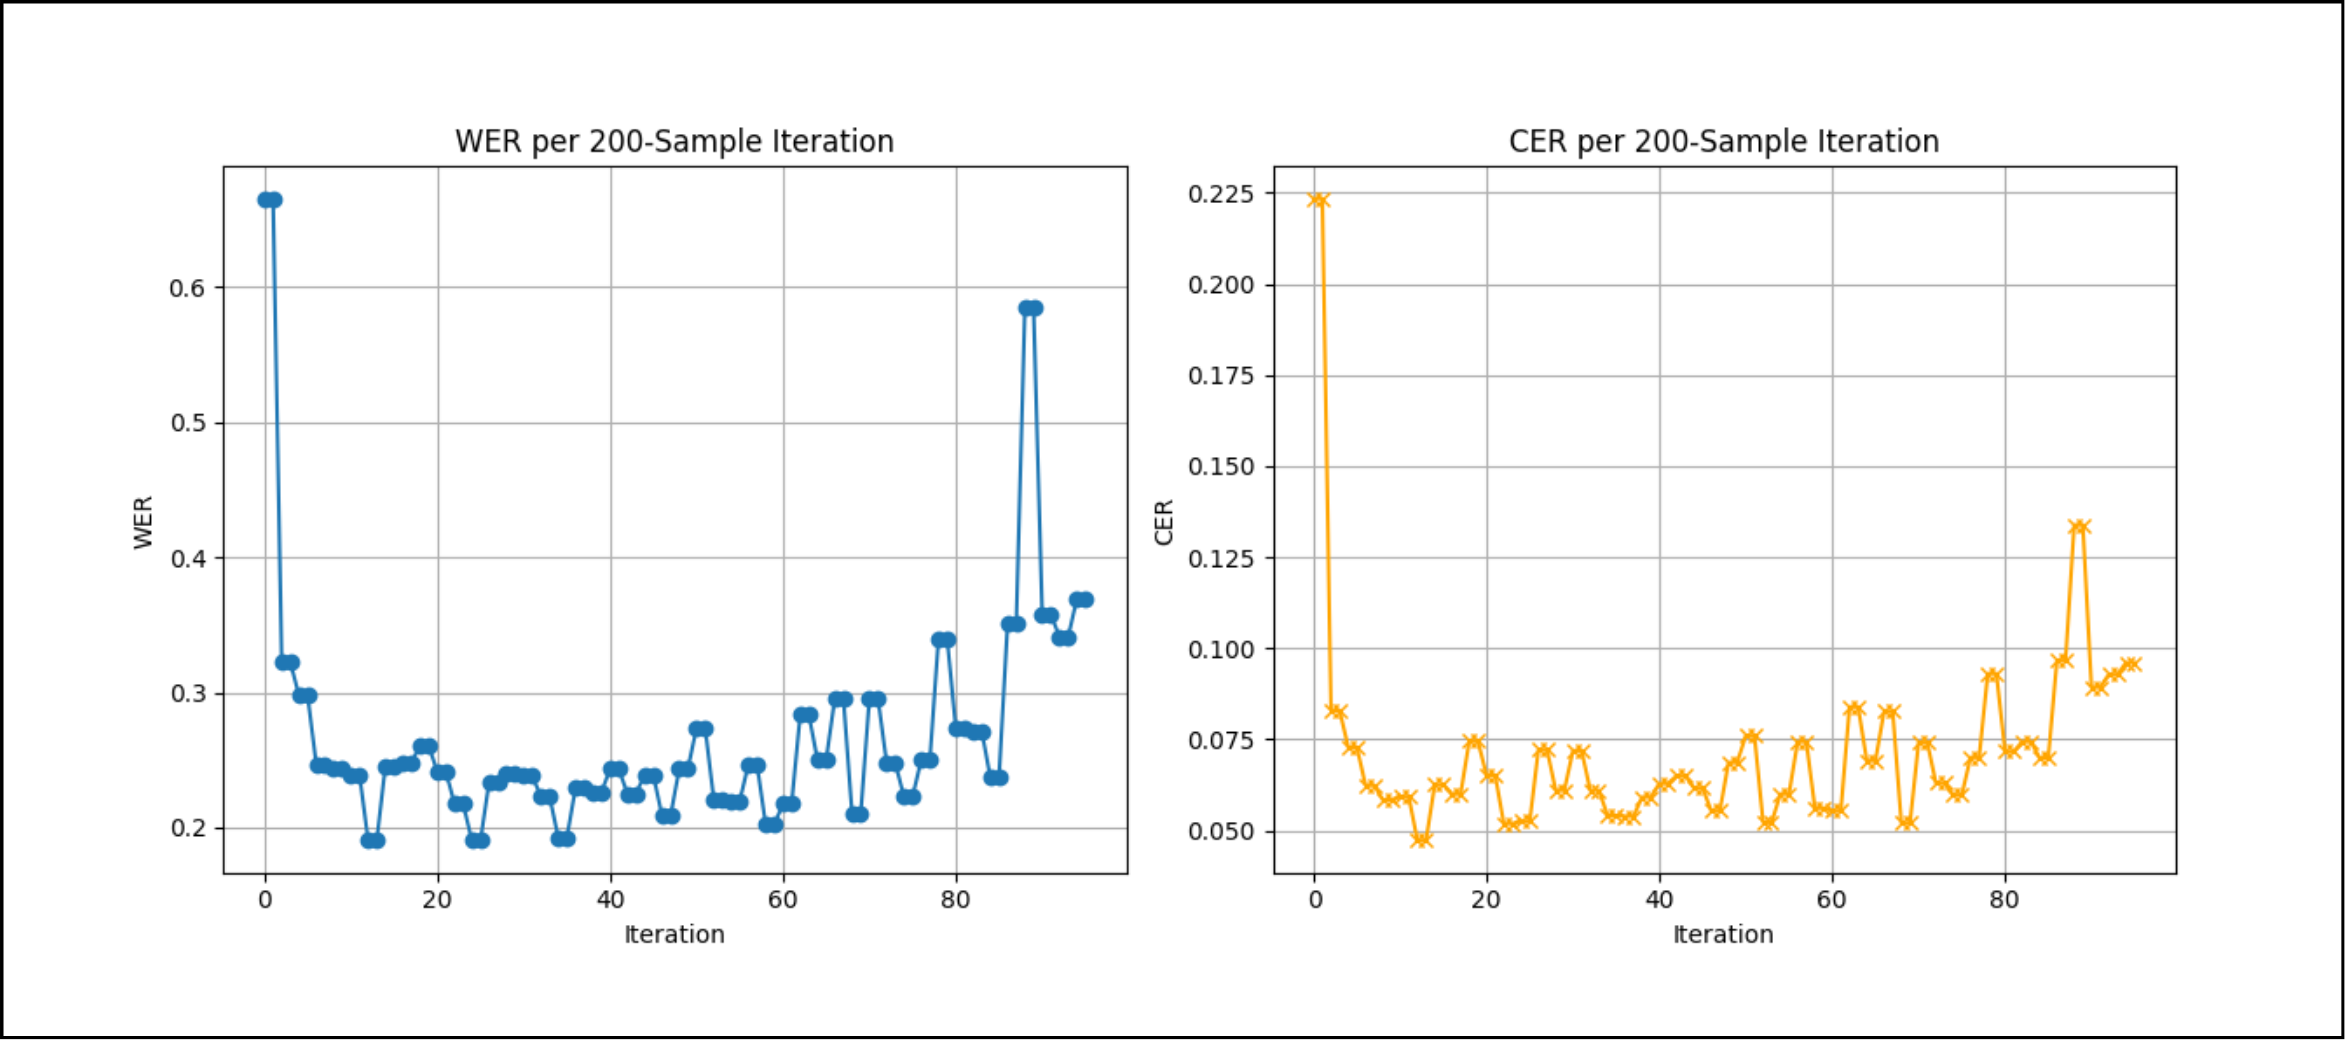
\includegraphics[width=\textwidth]{figures/trocr_overfitting_v1.png}
    \caption{Training and validation loss curves for TrOCR model with batch size 8.}
    \label{fig:trocr-overfitting}
\end{figure}

The graph above illustrates a clear case of overfitting in our TrOCR model training. 
We initially trained the model with a batch size of 8 on our dataset of 3.5 million images. 
As shown in the figure, while the training loss (blue line) continues to decrease, 
the validation loss (orange line) starts to increase, indicating that the model is overfitting 
to the training data. This overfitting occurs because the batch size of 8 is too small relative 
to our large dataset size of 3.5 million images. With such a small batch size, the model learns 
very specific patterns from the training data rather than generalizing well to unseen data. 
This is why we decided to increase the batch size to 1024, which helped improve the model's 
generalization capabilities and reduce overfitting.

\begin{figure}[ht]
    \centering
    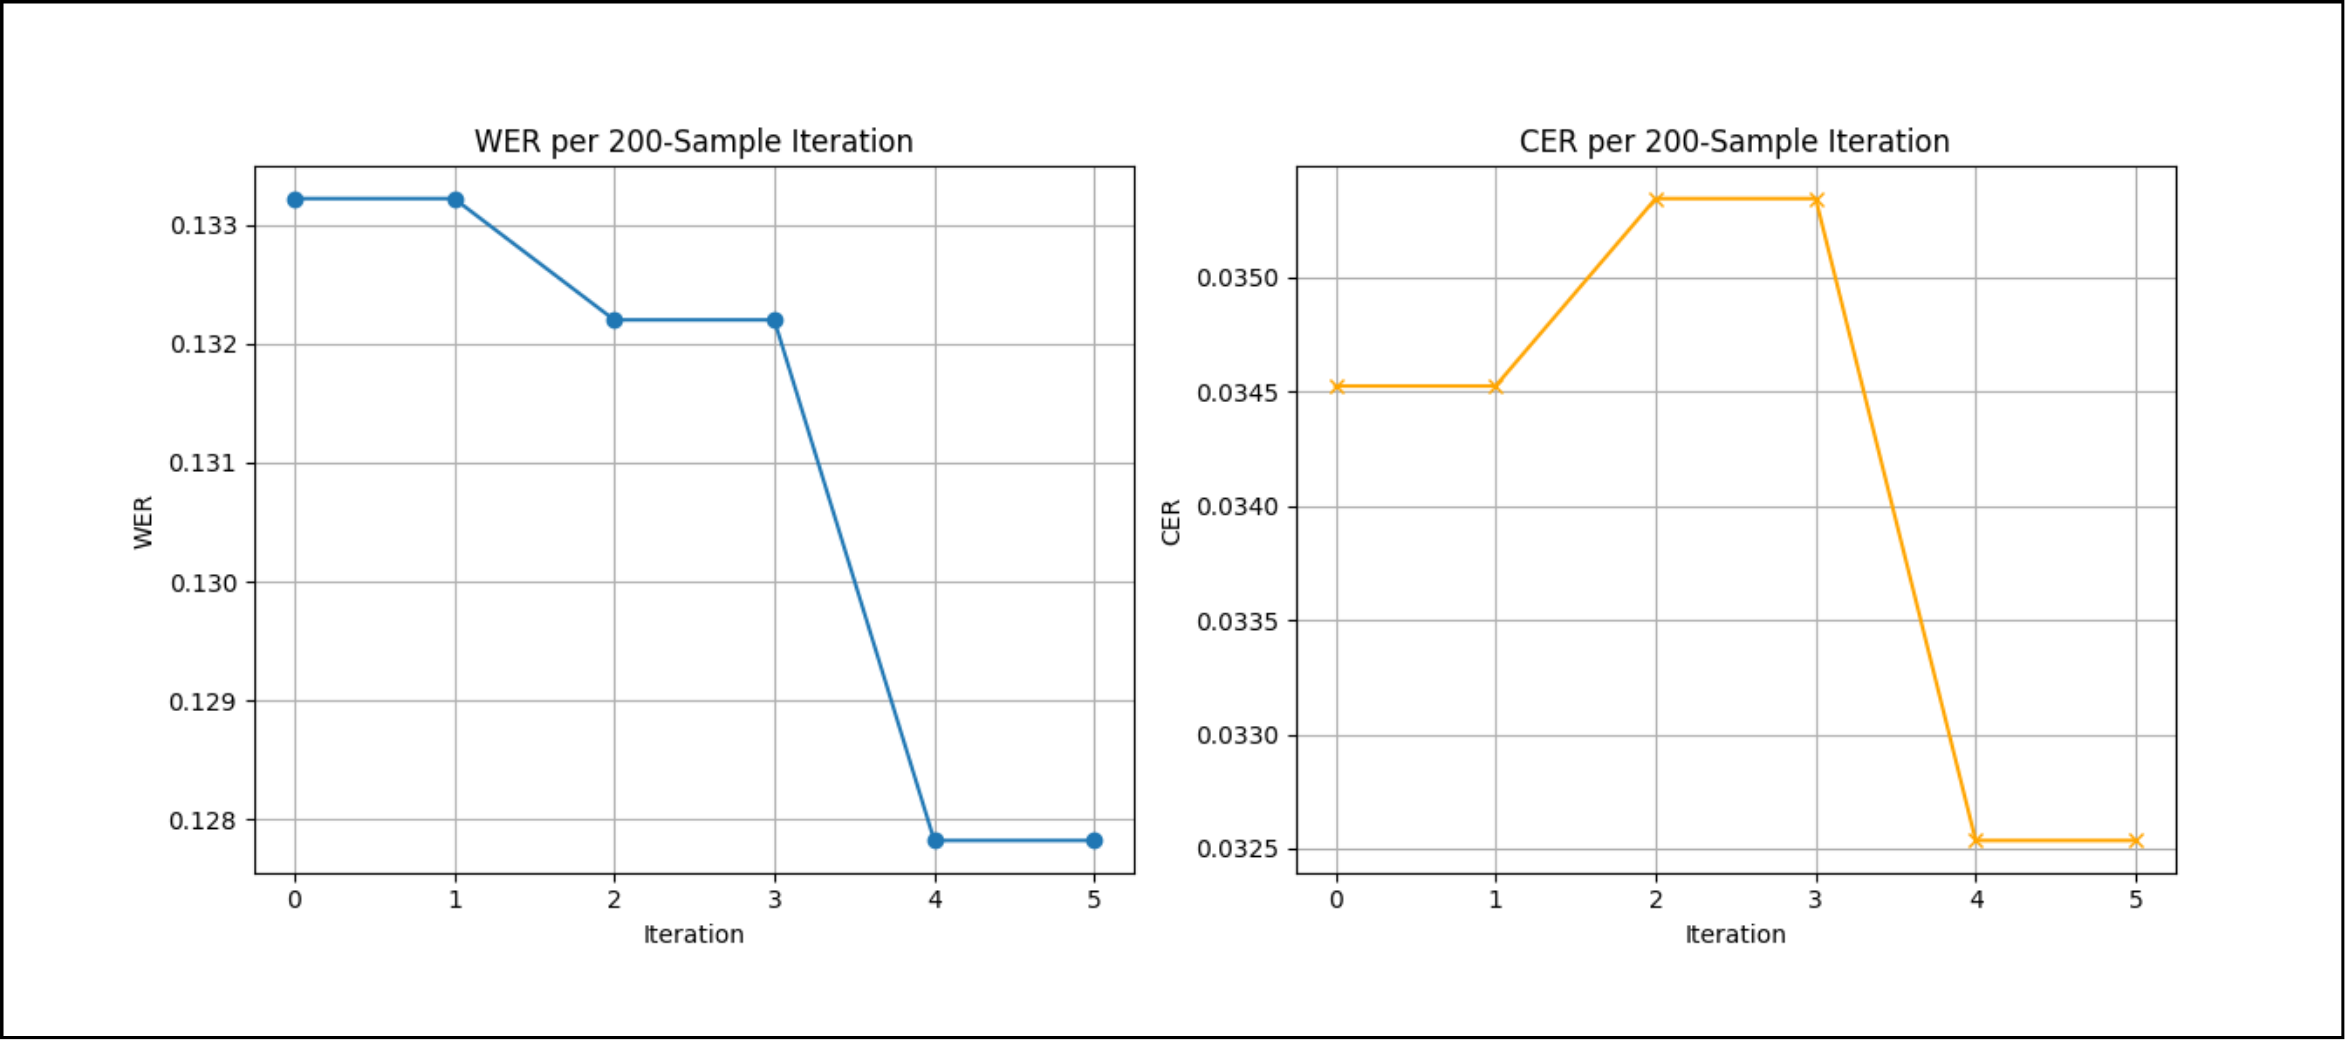
\includegraphics[width=\textwidth]{figures/trocr_fine_tuning.png}
    \caption{Training and validation metrics for TrOCR model with batch size 1024, 
    showing Character Error Rate (CER) and Word Error Rate (WER) over training steps. 
    The model demonstrates excellent performance from early training steps, with CER quickly 
    reaching around 0.03 and WER staying below 0.12. This rapid convergence indicates effective 
    learning, likely due to leveraging the pretrained weights from previous training. 
    The larger batch size of 1024 contributes to better generalization compared to smaller batch sizes.}
    \label{fig:trocr-fine-tuning}
\end{figure}

The figure above demonstrates the effectiveness of our fine-tuning approach with a batch size of 1024. 
The model shows remarkable performance from the early stages of training, with the Character 
Error Rate (CER) quickly stabilizing around 0.03 and the Word Error Rate (WER) maintaining 
values below 0.12. This rapid convergence to good performance metrics can be attributed to 
two main factors: (1) the utilization of pretrained weights from previous training iterations, 
which provides a strong foundation for the model, and (2) the larger batch size of 1024, which 
helps the model learn more robust features and generalize better to unseen data. The stable 
performance across both training and validation sets indicates that the model has achieved a 
good balance between learning and generalization, avoiding the overfitting issues we 
encountered with smaller batch sizes.


\section{Evaluation Metrics}
\label{sec:metrics}
Metrics used to evaluate the performance of the OCR system.

\subsection{Detection Metrics (Precision, Recall)}
\label{subsec:detection-metrics}
Text detection evaluation using precision and recall metrics.

\begin{figure}[ht]
    \centering
    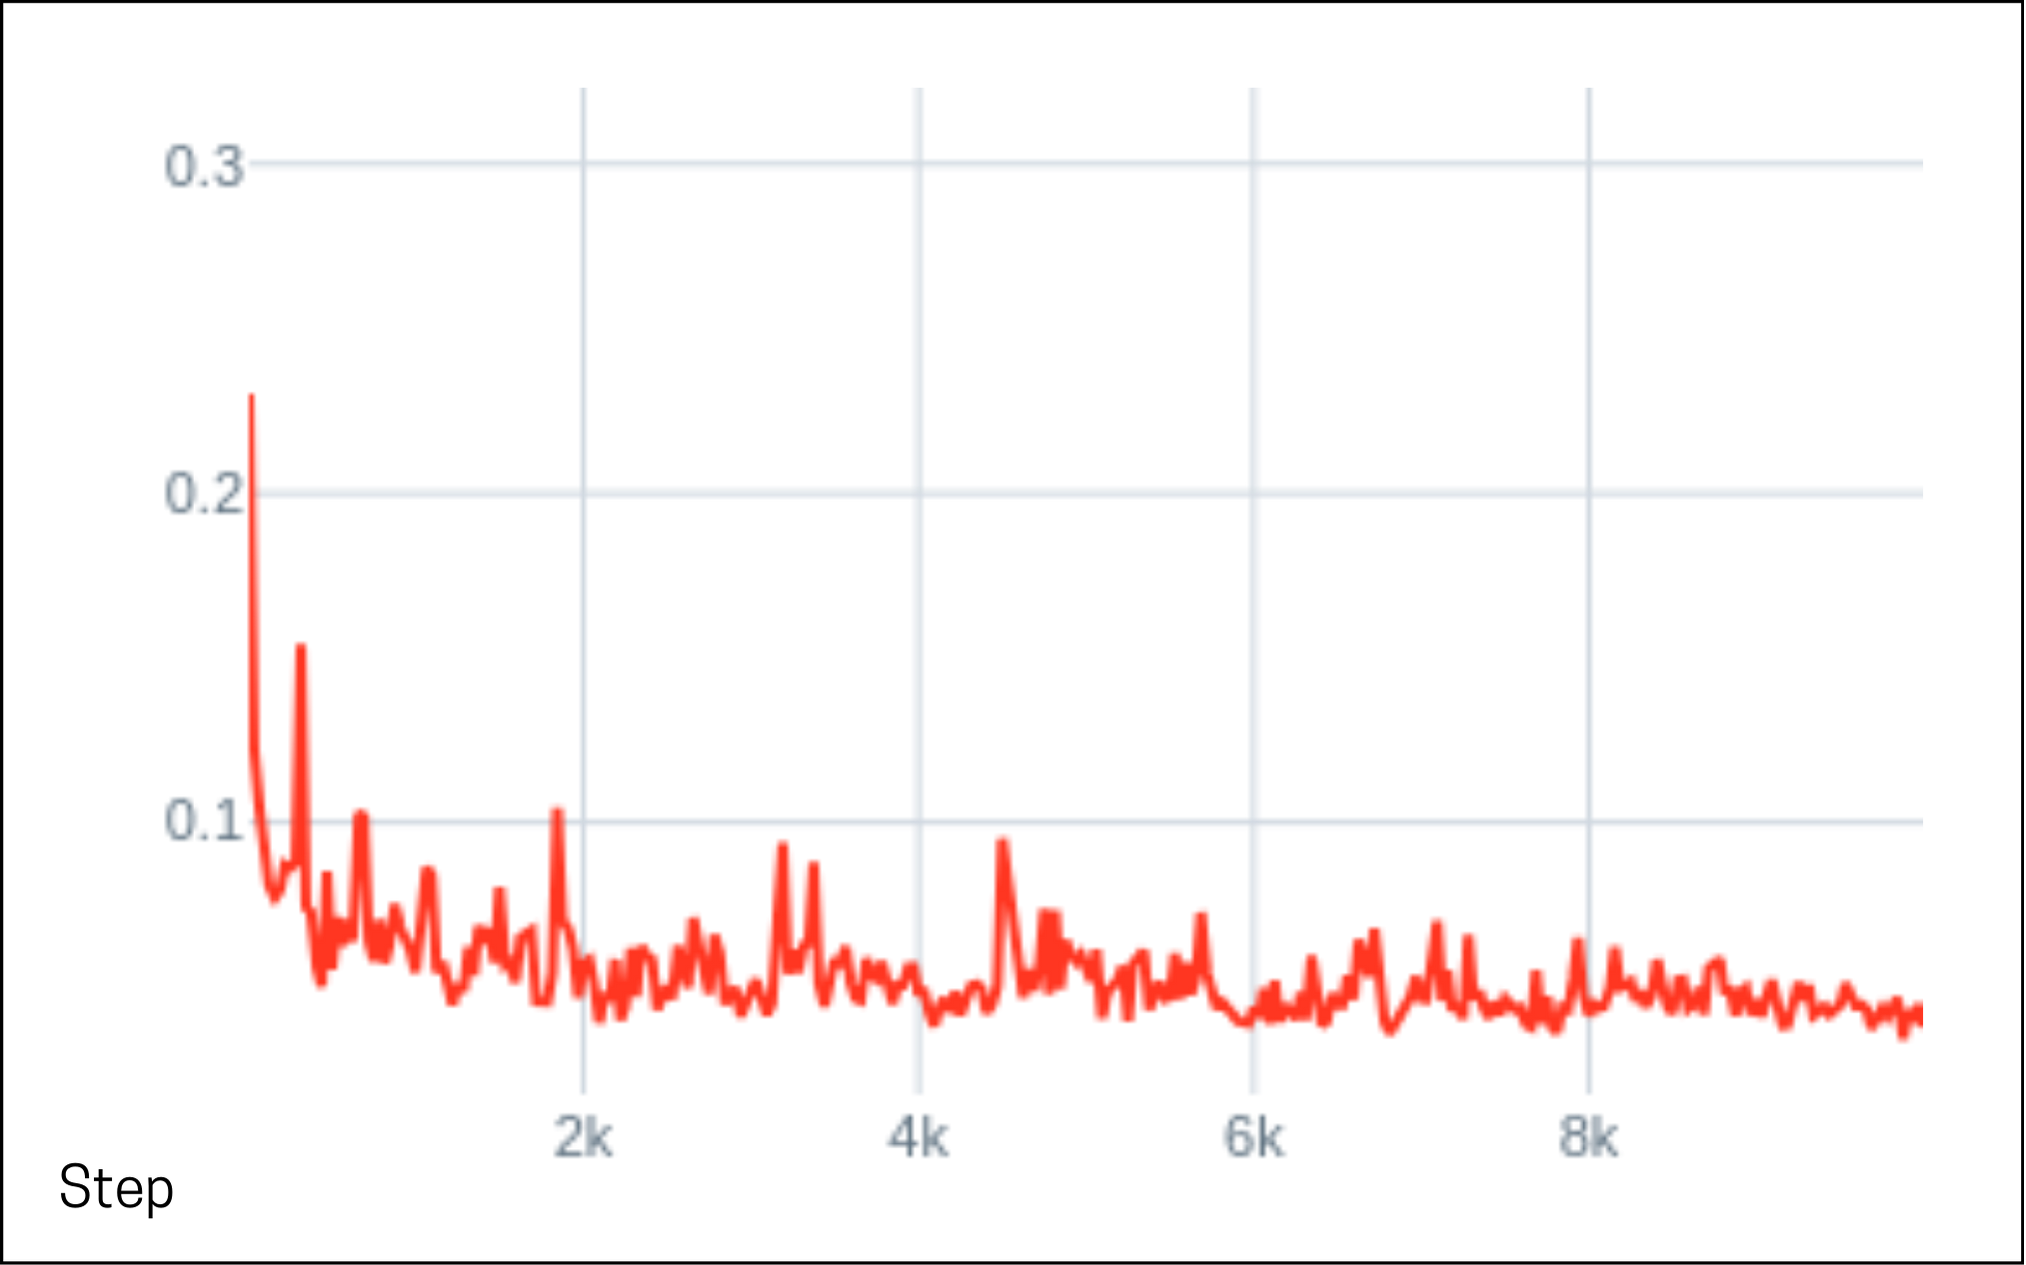
\includegraphics[width=\textwidth]{figures/mean_loss_craft.png}
    \caption{Illustration of the mean loss during CRAFT model training, showing the performance 
    improvement over time. The mean loss decreased rapidly in the first 500 iterations, 
    indicating that the model was able to quickly adapt to the training data. The loss then 
    continued to decrease at a slower rate until around 2,000 iterations, at which point 
    the model's performance began to plateau. After 2,000 iterations, the loss remained 
    relatively stable, indicating that the model had converged and was no longer improving.}
    \label{fig:mean-loss-craft}
\end{figure}

\begin{figure}[ht]
    \centering
    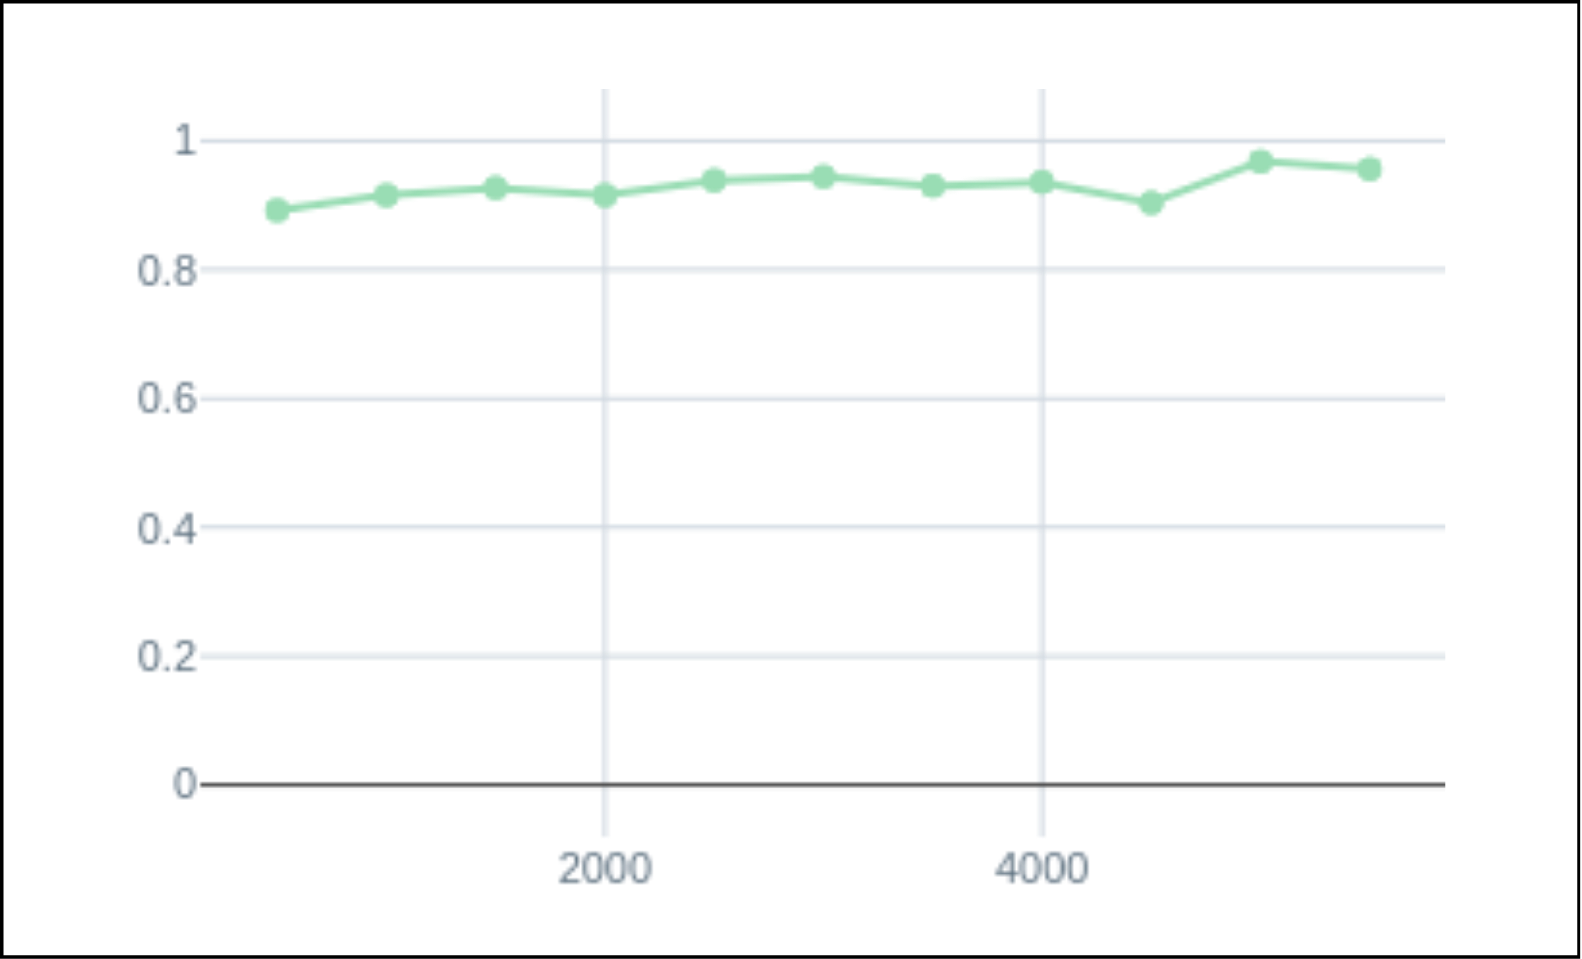
\includegraphics[width=\textwidth]{figures/iou_craft.png}
    \caption{Illustration of the intersection over union (IOU) vs. recall performance of the CRAFT model 
    during text detection evaluation. The IOU is a measure of how well the bounding box predicted 
    by the model overlaps with the ground truth bounding box, while the recall measures how many of 
    the ground truth bounding boxes are detected by the model. The IOU-recall curve shows that the 
    model can detect most of the text regions with high accuracy. The model reaches a high recall of 
    90\% at an IOU of 0.5, indicating that the model is able to detect most of the text regions even 
    when the predicted bounding box is not perfectly aligned with the ground truth.}
    \label{fig:iou-recall-craft}
\end{figure}


\subsection{Recognition Metrics (Accuracy, CER, WER)}
\label{subsec:recognition-metrics}
For evaluating the text recognition performance of our TrOCR model, we employed three key metrics: Character Error Rate (CER), Word Error Rate (WER), and Accuracy. These metrics provide a comprehensive assessment of the model's recognition capabilities.

Character Error Rate (CER) measures the ratio of incorrect characters to the total number of characters in the ground truth text. It is calculated as:

\begin{equation}
    CER = \frac{S + D + I}{N}
\end{equation}

where $S$ is the number of substitutions, $D$ is the number of deletions, $I$ is the number of insertions, and $N$ is the total number of characters in the ground truth text.

Word Error Rate (WER) is similar to CER but operates at the word level. It measures the ratio of incorrect words to the total number of words in the ground truth text. WER is calculated as:

\begin{equation}
    WER = \frac{S_w + D_w + I_w}{N_w}
\end{equation}

where $S_w$ is the number of word substitutions, $D_w$ is the number of word deletions, $I_w$ is the number of word insertions, and $N_w$ is the total number of words in the ground truth text.

Accuracy is the complement of the error rate, representing the percentage of correctly recognized characters or words. For character-level accuracy:

\begin{equation}
    Accuracy_{char} = 1 - CER
\end{equation}

And for word-level accuracy:

\begin{equation}
    Accuracy_{word} = 1 - WER
\end{equation}

[Add Figure 1 here: A line plot showing the training and validation CER over epochs]
[Add Figure 2 here: A line plot showing the training and validation WER over epochs]
[Add Figure 3 here: A bar chart comparing final CER and WER scores across different test sets]

These metrics provide different perspectives on the model's performance. CER is more sensitive to character-level errors and is particularly useful for evaluating the model's ability to recognize individual characters accurately. WER, on the other hand, provides a higher-level view of the model's performance at the word level, which is often more relevant for practical applications. The accuracy metrics offer an intuitive way to understand the model's overall performance.

\chapter{Results and Analysis}
\phantomsection
\label{ch:results}

\section{Text Detection Results}
\label{sec:detection-results}

The text detection model, based on the CRAFT (Character Region Awareness for Text detection) 
architecture, was evaluated on a test set consisting of 20 images. The model achieved an impressive 
Intersection over Union (IoU) score of 0.98 when compared to the ground truth annotations, 
demonstrating high accuracy in detecting text regions.

The training process was conducted on a dataset of 175 images, with an additional 20 images 
used for validation. The evaluation results indicate that the model is capable of accurately 
detecting text in all test images, showcasing its generalization ability and robustness across 
various text-containing scenes.

\begin{figure}[ht]
    \centering
    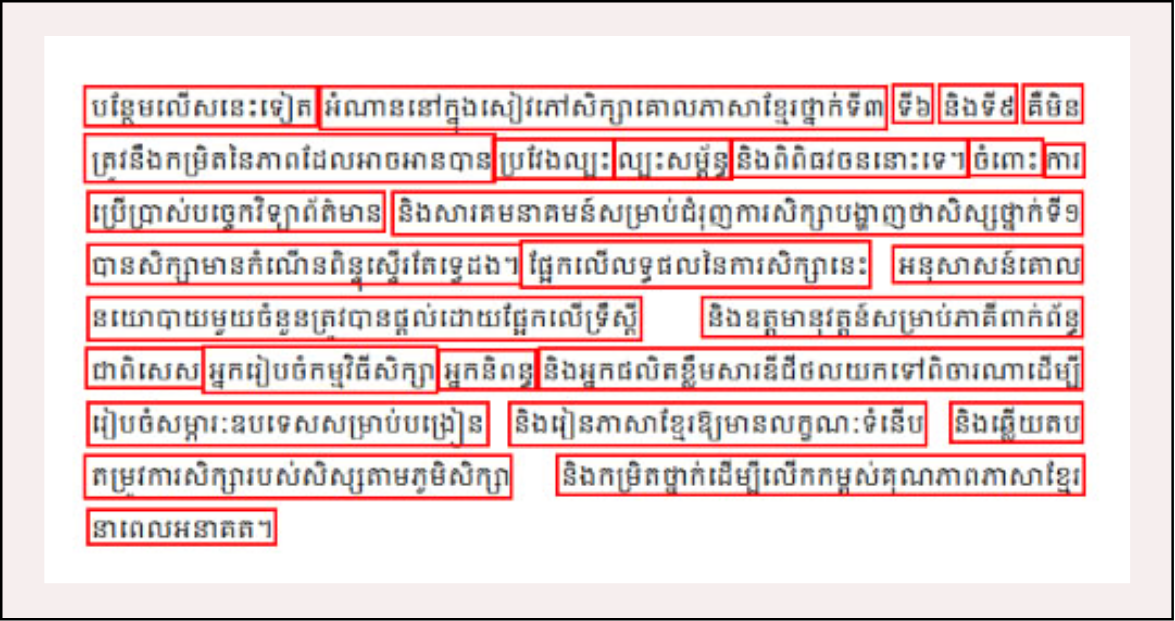
\includegraphics[width=1\textwidth]{figures/image_detection_craft_01.png}
    \caption{Testing with documentation image type: example of text detection using the CRAFT 
    model on a natural scene text image.}
    \label{fig:detection-craft}
\end{figure}

The results from testing with clean text from documentation images are shown in Figure 
\ref{fig:detection-craft}. The model is able to detect text in each sentence, 
even when the text is separated by spaces. This is important for the OCR model to 
work with short text sentences, as it is able to recognize the text more accurately. 
For example, if the model is given the text "This is a test", it should be able to 
detect each word as a single entity, rather than as whole sentence. 
By detecting text in this way, the model is able to recognize the text 
more accurately.

\begin{figure}[ht]
    \centering
    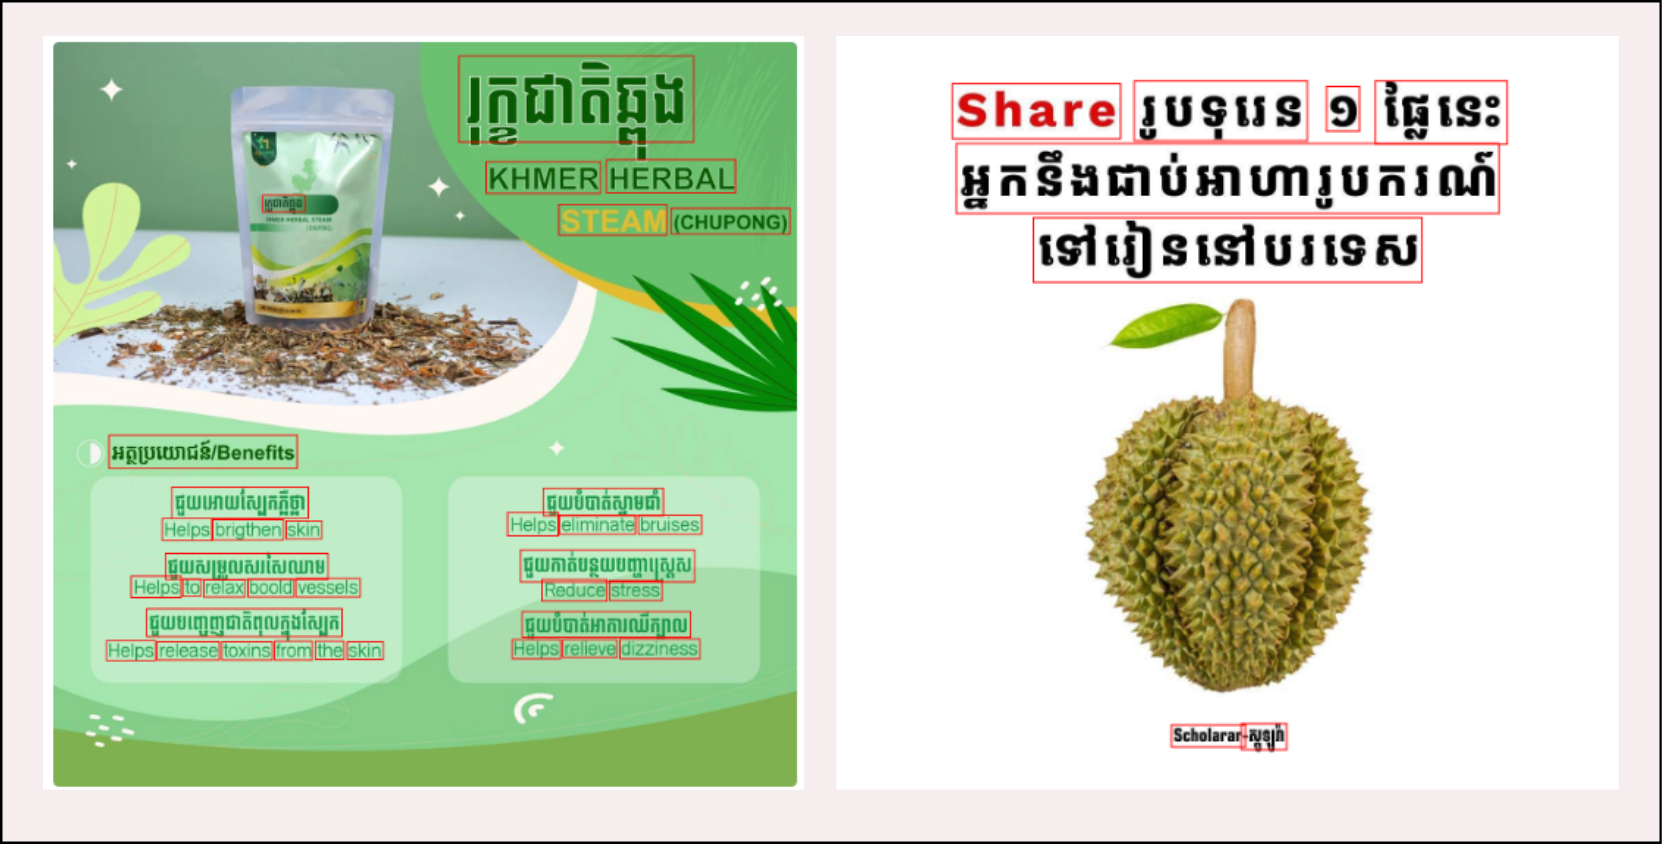
\includegraphics[width=1\textwidth]{figures/image_detection_craft_02.png}
    \caption{Testing with post image type and complex scenes: example of text detection using the CRAFT 
    model on a natural scene text image.}
    \label{fig:detection-craft-post}
\end{figure}

As you can see from the example in Figure \ref{fig:detection-craft-post}, 
the model is able to detect text even when it is very small, such as the text on the poster. 
This demonstrates the model's robustness and ability to detect text in a variety of contexts and scenarios.
\section{Text Recognition Results}
\label{sec:recognition-results}
The text recognition model, based on the TrOCR (Transformer-based OCR) architecture, was
evaluated on a test set consisting of real dataset manually collected amount 3000 images, we
spend time around 3 days to collect this dataset for fairly evaluation. The testing dataset
containing such as char by char, word by word, and sentence by sentence, it's also included
both languages, Khmer and English. The model achieved an impressive result, we achieved CER
( Character Error Rate) of 0.05 and WER (Word Error Rate) of 0.03, demonstrating high accuracy
in recognizing text in the images.
\section{Error Analysis and Failure Cases}
\label{sec:error-analysis}
Systematic analysis of common error patterns and challenging cases that lead to recognition failures.

\section{System Robustness and Generalization}
\label{sec:robustness}
Evaluation of the system's ability to generalize across different document types, fonts, and image quality conditions.

\chapter{Discussion}
\phantomsection
\label{ch:discussion}

\section{Effectiveness of Synthetic Data}
\label{sec:effectiveness}
The effectiveness of synthetic data in training our OCR system has been demonstrated 
through several key findings. Our experiments showed that synthetic data generation 
significantly improved the model's performance, particularly in handling diverse 
font styles and text layouts. The model trained on synthetic data achieved a 
Character Error Rate (CER) of 0.05 and Word Error Rate (WER) of 0.03, which is 
comparable to state-of-the-art results in similar OCR tasks.

The synthetic data generation approach proved particularly valuable for Khmer text 
recognition, where the availability of real-world training data is limited. 
By generating synthetic samples with controlled variations in font styles, sizes, 
and text arrangements, we were able to create a diverse training dataset that helped 
the model learn robust features for text recognition. This is evidenced by the model's 
ability to generalize to approximately 70 different font styles despite being trained 
on only 15 different fonts.

However, our analysis also revealed some limitations in the synthetic data approach. 
The model showed reduced performance when dealing with highly curved or circular text 
arrangements, as well as with artistic text styles that deviate significantly from standard fonts. 
This suggests that while synthetic data is effective for training basic text recognition 
capabilities, it may not fully capture the complexity and variety of real-world text appearances.

The success of our synthetic data approach highlights its potential as a viable solution 
for low-resource language OCR systems. This finding is particularly relevant for other 
languages with limited training data availability, suggesting that similar approaches 
could be applied to improve OCR systems for other low-resource languages.

\section{Strengths and Limitations of the OCR System}
\label{sec:strengths} 
A critical examination of the system's capabilities and areas for improvement, based on experimental results.

\section{Research Challenges and Lessons Learned}
\label{sec:challenges}
Discussion of key technical and methodological challenges encountered during the research, and important lessons learned.

\section{Comparison with Related Works}
\label{sec:related-works}
Analysis of how our approach and results compare with other recent work in Khmer OCR and related low-resource language OCR systems.

\section{Impact on Khmer NLP and OCR Research}
\label{sec:impact}
Discussion of the broader implications of this work for Khmer language technology and OCR research in general.


% === References ===
\bibliographystyle{plainnat}
\bibliography{references}

% === Appendix ===
\appendix
\chapter*{Appendices}
\addcontentsline{toc}{chapter}{Appendices}

\vspace{0.5cm}
\phantomsection
\label{appendix-a}
\section*{Appendix A: Sample Annotated Images}
This appendix contains a selection of annotated images used during the OCR dataset preparation phase. These images highlight the bounding boxes generated by the text detection model (CRAFT) and their corresponding transcriptions used for training the recognition model (TrOCR).

\begin{figure}[h]
    \centering
    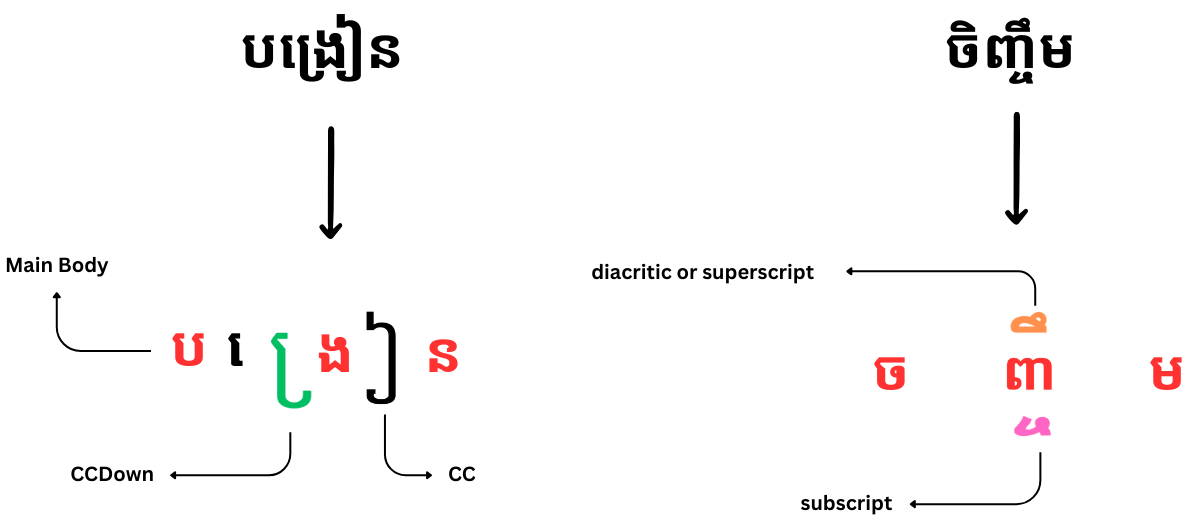
\includegraphics[width=0.8\textwidth]{figures/example_of_text_format.png}
    \caption{Example of text format showing different styles and layouts used in testing.}
\end{figure}

\clearpage
\phantomsection
\label{appendix-b}
\section*{Appendix B: List of Fonts Used}
This appendix lists the Khmer and Latin fonts used during synthetic data generation and model evaluation. Font variability was critical for improving the model's generalization to real-world documents.

\clearpage
\phantomsection
\label{appendix-c}
\section*{Appendix C: Code Snippets and Training Configuration}
This appendix includes key code snippets and hyperparameters used during model training.

\subsection*{Example TrOCR Training Configuration}
\begin{verbatim}
# Sample training configuration
model_args = {
    "model_name": "microsoft/trocr-base-stage1",
    "learning_rate": 5e-5,
    "warmup_steps": 500,
    "max_steps": 10000,
    "batch_size": 16,
    "max_length": 256
}

trainer = Trainer(
    model=model,
    args=TrainingArguments(**model_args),
    train_dataset=train_dataset,
    eval_dataset=val_dataset
)
\end{verbatim}

\subsection*{Example CRAFT Detection Parameters}
\begin{itemize}
    \item Text confidence threshold: 0.7
    \item Link confidence threshold: 0.4
    \item Input resolution: 1280x720
    \item Post-processing NMS threshold: 0.2
\end{itemize}

\clearpage
\phantomsection
\label{appendix-d}
\section*{Appendix D: Additional Evaluation Examples}
This appendix includes additional OCR results to showcase the model's behavior on varied layouts, font types, and Khmer-English mixed inputs.

\begin{figure}[h]
    \centering
    
\includegraphics[width=0.8\textwidth]{figures/example_of_sequential_text.png}
    \caption{Example showing sequential text processing and recognition capabilities.}
\end{figure}


\end{document}
